\subsection{Chapter 13 - Waves}

\subsubsection{Overview}\label{chapter:waves}

In this chapter we introduce the tools to describe waves. Waves arise in many different physical systems (the ocean, a string, electromagnetism, etc.), and can be described by a common mathematical framework.

\begin{framed}
\textbf{Learning Objectives}\\
\begin{itemize}
\item Understand the definition of different types of waves.
\item Understand how to mathematically describe travelling and standing waves.
\item Understand how to model the propagation of a pulse on a rope.
\item Understand how to model the energy transported by a wave.
\item Understand how to model the interference of waves.
\item Understand how standing waves form and how to model them.
\end{itemize}
\end{framed}

\begin{framed}
\textbf{Think About It}\\
Two waves travel down two identical strings (Figure~\ref{fig:waves:opening}). The frequency of the first wave is twice that of the second wave. Which wave will be faster?

\begin{figure}[!htbp]
\centering
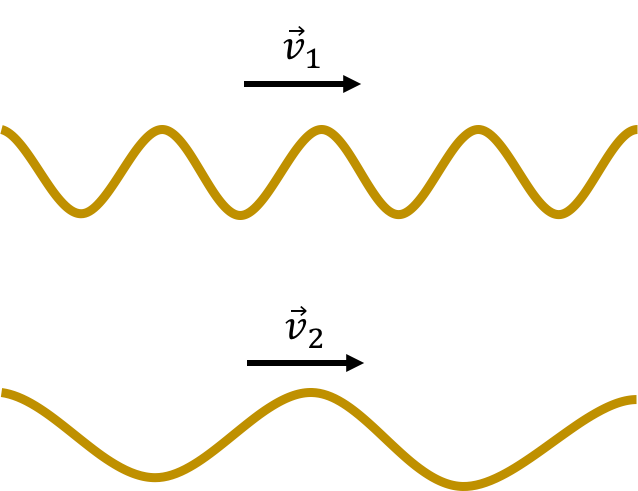
\includegraphics[width=0.3\linewidth]{files/wavevel-074d8cd41f9c5ee4879fb1b851f99323.png}
\caption[]{Two waves travelling down two identical strings.}
\label{fig:waves:opening}
\end{figure}

\begin{enumerate}
\item The first wave.
\item The second wave.
\item The speeds will be the same.
\end{enumerate}

\begin{framed}
\textbf{Answer}\\
\begin{enumerate}[resume]
\item
\end{enumerate}
\end{framed}
\end{framed}

\subsubsection{Characteristics of a wave}

\paragraph{Definition and types of waves}

A travelling wave is a \textbf{disturbance that travels through} a medium. Consider the waves made by fans at a soccer game, as in Figure~\ref{fig:waves:soccer}.
The fans can be thought of as the medium through which the wave propagates. The elements of the medium may oscillate about an equilibrium position (the fans move a short distance up and down), but they do not travel with the wave (the fans do not move horizontally with the wave).

\begin{figure}[!htbp]
\centering
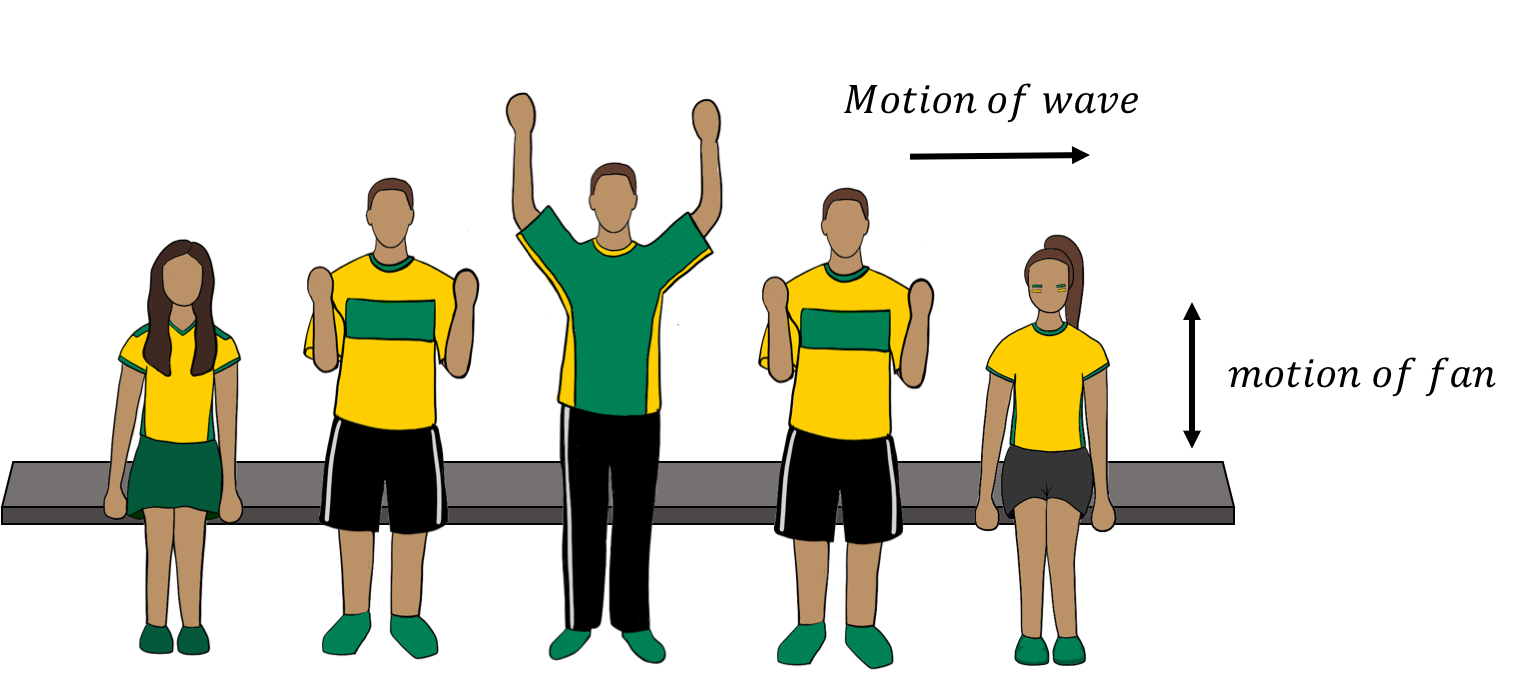
\includegraphics[width=0.8\linewidth]{files/soccer-09bc9ff0a701ec33a391b979a7f81fbf.png}
\caption[]{A transverse wave made by soccer fans moving up and down.}
\label{fig:waves:soccer}
\end{figure}

Consider the ripples (waves) made by a rock dropped in a pond (Figure~\ref{fig:waves:water}). The ripples travel outwards from where the rock was dropped, but the water itself does not move outwards. The individual water molecules will move in small circles about an equilibrium position, but they do not move along with the waves.

\begin{figure}[!htbp]
\centering
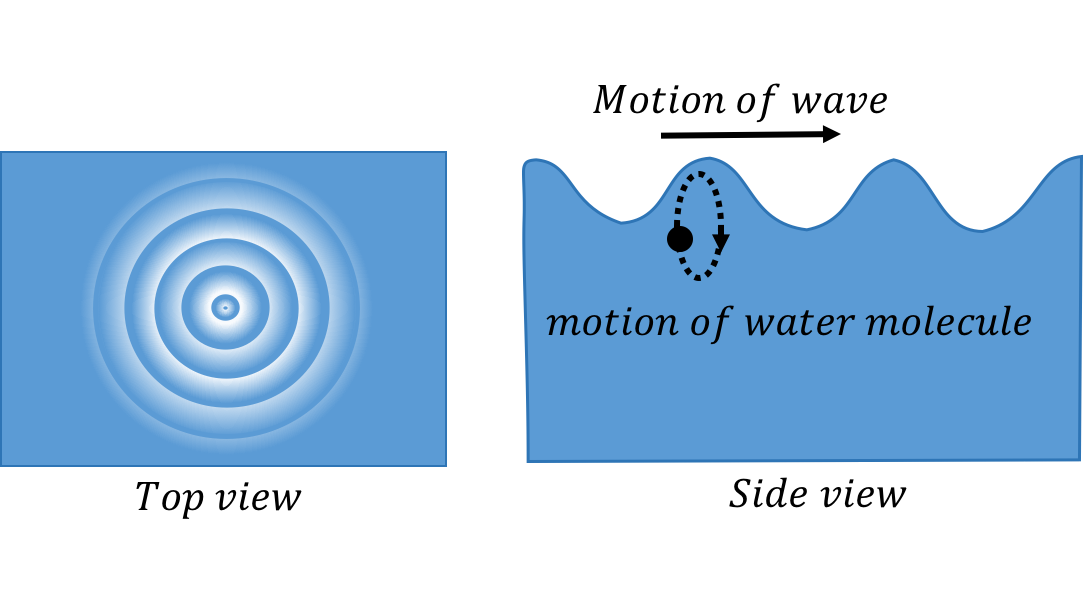
\includegraphics[width=0.6\linewidth]{files/water-fcfb7b7981c2ab5310c1575077308bf3.png}
\caption[]{A transverse wave travelling through water. The left panel shows the view from above as ripples move outwards. The right panel shows the motion of an individual water molecule as the wave is viewed from the side.}
\label{fig:waves:water}
\end{figure}

We can distinguish between two classes of waves, based on the motion of the medium through which it propagates. With \textbf{transverse waves}, the elements of the medium oscillate back and forth in a direction perpendicular to the motion of the wave. For example, if you attach a horizontal rope to a wall and move the other end up and down (Figure~\ref{fig:waves:rope}), you can create a disturbance (a wave) that travels horizontally along the rope. The parts of the rope do not move horizontally; they only move up and down, about some equilibrium position.

\begin{figure}[!htbp]
\centering
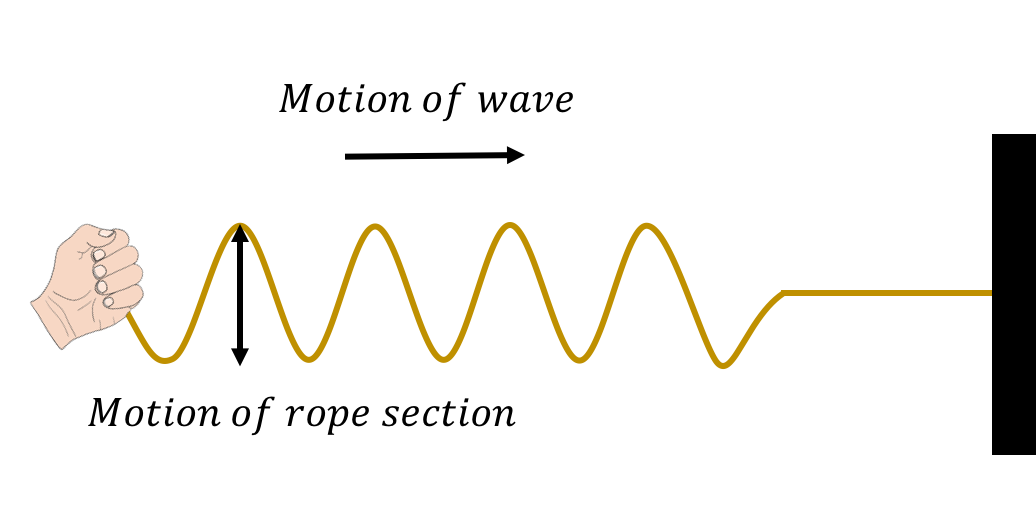
\includegraphics[width=0.6\linewidth]{files/rope-0b107780d3edd953a01b4e92cb37aad2.png}
\caption[]{A transverse wave travelling through a rope. The wave is created by moving one end of the rope up and down.}
\label{fig:waves:rope}
\end{figure}

With \textbf{longitudinal waves}, the elements of the medium oscillate back and forth in the same direction as the motion of the wave. If you clap your hands, you will create a pressure disturbance in the air that will propagate; this is what we call sound (a sound wave). The air molecules oscillate about an equilibrium position in the same direction as the wave propagates, but they do not move with the wave.

\begin{figure}[!htbp]
\centering
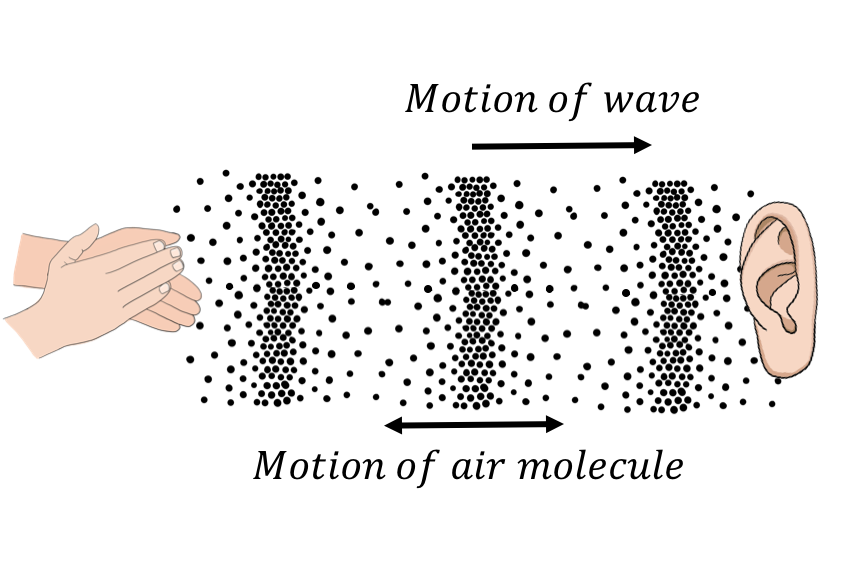
\includegraphics[width=0.6\linewidth]{files/sound-13b08117b78a8ef141b2742713c472cf.png}
\caption[]{A longitudinal sound wave travelling through the air. The air molecules move back and forth in the same direction as the wave, but they oscillate about an equilibrium position instead of moving with the wave.}
\label{fig:waves:sound}
\end{figure}

Furthermore, we can distinguish between ``travelling waves'', in which a disturbance propagates through a medium, and ``standing waves'', which do not transport energy through the medium (for example, a vibrating string on a violin).

\begin{framed}
\textbf{Checkpoint}\\
Are the waves propagating through a slinky when you compress and elongate it (Figure~\ref{fig:waves:slinky}) transverse or longitudinal?

\begin{figure}[!htbp]
\centering
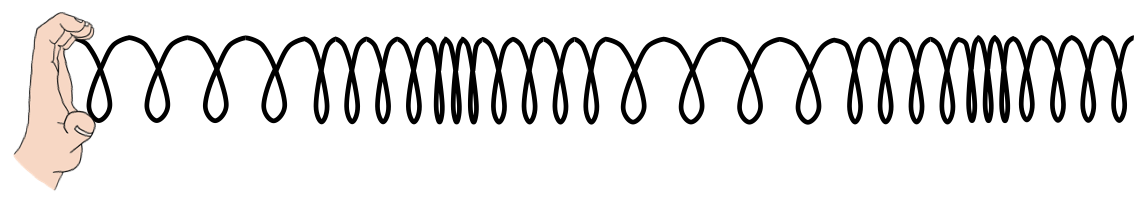
\includegraphics[width=0.6\linewidth]{files/slinky-dbf6d8004be443a3d11451ea867b4f98.png}
\caption[]{A wave travelling through a slinky. The wave is created when you compress or elongate the slinky.}
\label{fig:waves:slinky}
\end{figure}

\begin{enumerate}
\item Transverse
\item Longitudinal
\end{enumerate}

\begin{framed}
\textbf{Answer}\\
\begin{enumerate}[resume]
\item
\end{enumerate}
\end{framed}
\end{framed}

Physically, a wave can only propagate through a medium if the medium can be deformed. When a particle in the medium is disturbed from its equilibrium position, it will experience a restoring force that acts to bring it back to its equilibrium position. Often, if the displacement of the particle from the equilibrium is small, the magnitude of that force is proportional to the displacement. Thus, as we will see, we can model the propagation of waves by treating the particles in the medium as simple harmonic oscillators.

A source of energy is required in order to deform the medium and generate a wave. For example, that source of energy could be a speaker creating sound waves by pushing a membrane back and forth; speakers require energy, and are often rated by the electrical power that they convert into sound waves (e.g. a $50 {\rm W}$ speaker consumes $50 {\rm W}$ of electrical power to produce sound).

\begin{figure}[!htbp]
\centering
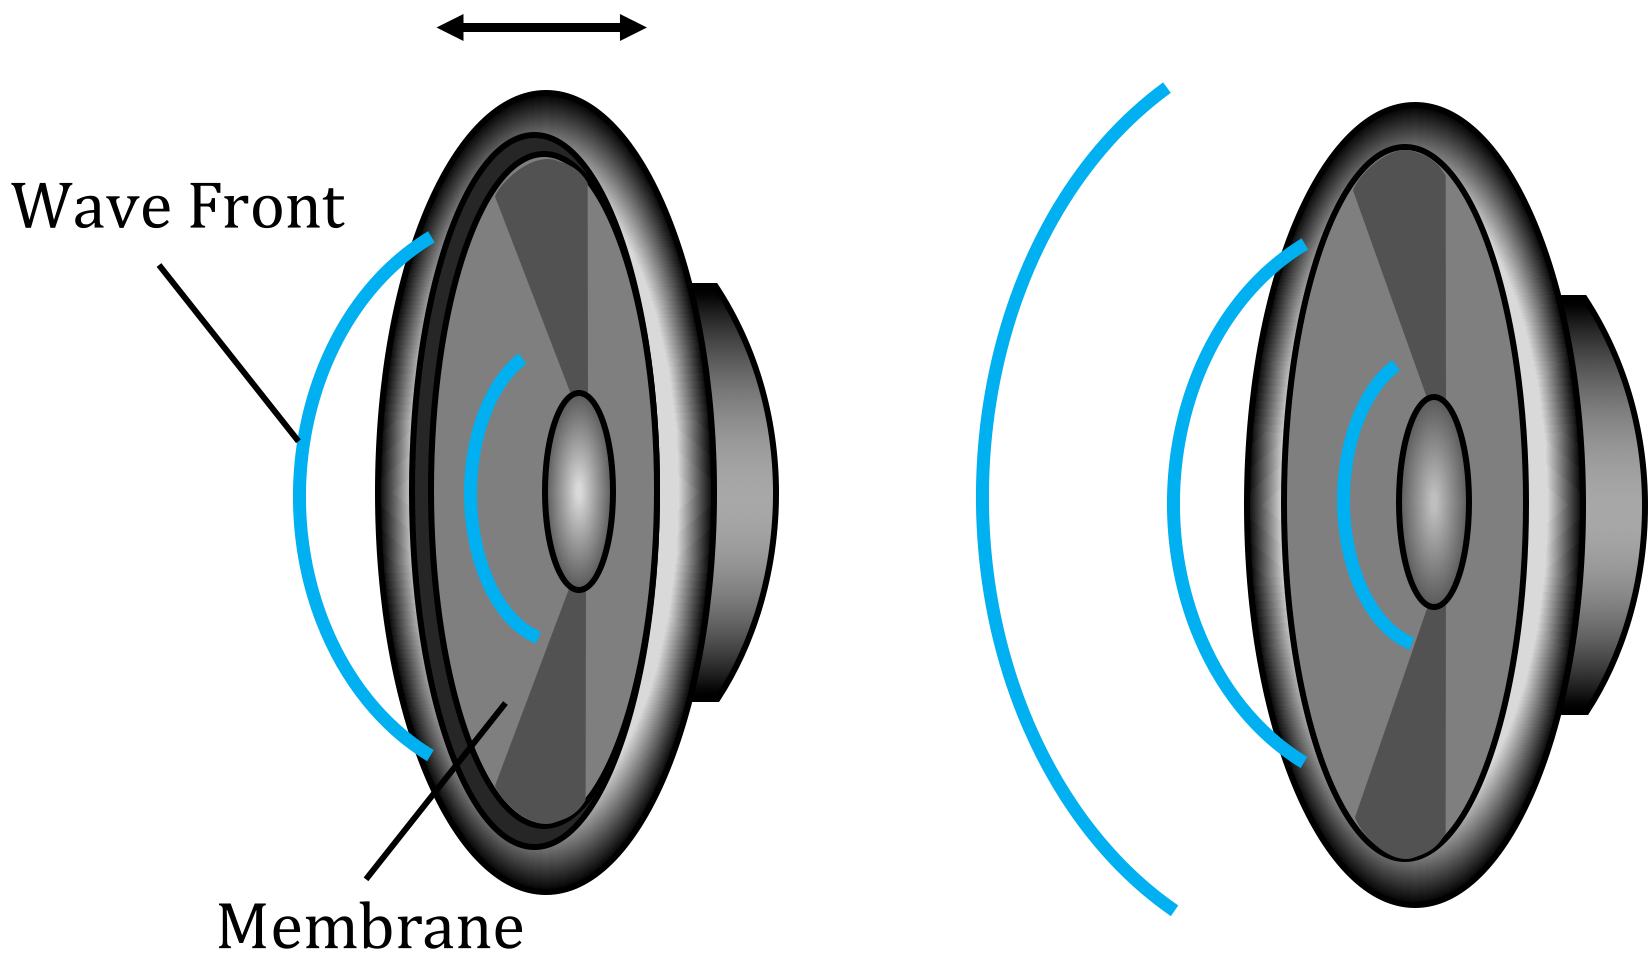
\includegraphics[width=0.6\linewidth]{files/speaker-3abc5643ad51e7f35ed507b362ea47e3.png}
\caption[]{A speaker creating sound waves. The membrane vibrates back and forth which deforms the air to create sound waves that propagate through the air.}
\label{fig:waves:speaker}
\end{figure}

\paragraph{Description of a wave}

In this chapter, we will mostly discuss how to describe sinusoidal waves; those for which the displacement of particles in the medium can be described by a sinusoidally-varying function of position. As we will see, more complicated waves can always be described as if they are the combination of multiple sine waves. We can use several quantities to describe a travelling wave, which are illustrated in Figure~\ref{fig:waves:wavelength}:

\begin{itemize}
\item The \textbf{wavelength}, $\lambda$, is the distance between two  successive maxima (``peaks'') or minima (``troughs'') in the wave.
\item The \textbf{amplitude}, $A$, is the maximal distance that a particle in the medium is displaced from its equilibrium position.
\item The \textbf{velocity}, $\vec v$, is the velocity with which the disturbance propagates through the medium.
\item The \textbf{period}, $T$, is the time it takes for two successive maxima (or minima) to pass through the same point in the medium.
\item The \textbf{frequency}, $f$, is the inverse of the period ($f=1/T$).
\end{itemize}

\begin{figure}[!htbp]
\centering
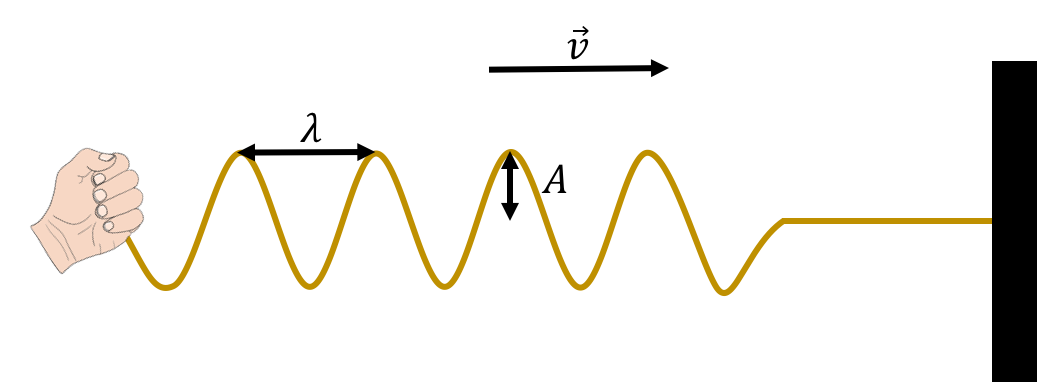
\includegraphics[width=0.6\linewidth]{files/wavelength-712d212633d75161a04c533bf9ec7922.png}
\caption[]{Wavelength, velocity, and amplitude for a transverse wave on a rope.}
\label{fig:waves:wavelength}
\end{figure}

The wavelength, speed, and period of the wave are related, since the amount of time that it takes for two successive maxima of the wave to pass through a given point will depend on the speed of the wave and the distance between maxima, $\lambda$. Since it takes a time, $T$, for two maxima a distance $\lambda$ apart to pass through a given point in the medium, the speed of the wave is given by:
\begin{equation}
\label{eq:waves:speed}
\boxed{v = \frac{\lambda}{T}=\lambda f}
\end{equation}
Thus, of the three quantities (speed, period/frequency, and wavelength), only two are independent, as the third quantity must depend on the value of the other two. \textbf{The speed of a wave depends on the properties of the medium through which the wave propagates and not on the mechanism that is generating the wave}. For example, the speed of sound waves depends on the pressure, density, and temperature of the air through which they propagate, and not on what is making the sound. When a mechanism generates a wave, that mechanism usually determines the frequency of the wave (e.g. frequency with which the hand in Figure~\ref{fig:waves:wavelength} moves up and down), the speed is determined by the medium, and the wavelength can be determined from (\ref{eq:waves:speed}).

\begin{framed}
\textbf{Checkpoint}\\
What can you say about the sound emitted by a cello versus that emitted by a violin?\}

\begin{enumerate}
\item The sound from the violin has a higher frequency.
\item The sound from the cello has a longer wavelength.
\item The sound from both instruments propagates at the same speed.
\item All of the above.
\end{enumerate}

\begin{framed}
\textbf{Answer}\\
\begin{enumerate}[resume]
\item
\end{enumerate}
\end{framed}
\end{framed}

\subsubsection{Mathematical description of a wave}

In order to describe the motion of a wave through a medium, we can describe the motion of the individual particles of the medium as the wave passes through. Specifically, we describe the position of each particle using its displacement, $D$, from its equilibrium position. Consider our rope example in which a sine wave is propagating through a medium (the rope) in the positive $x$ direction, as shown in Figure~\ref{fig:waves:sinewaveaxes}

\begin{figure}[!htbp]
\centering
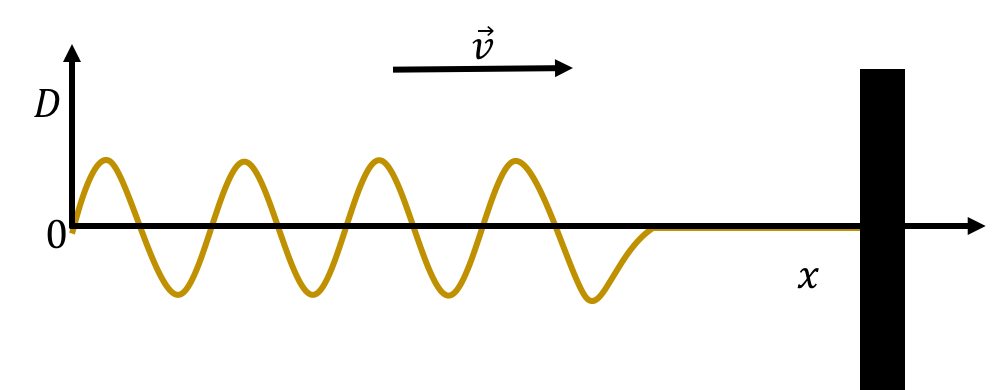
\includegraphics[width=0.6\linewidth]{files/sinewaveaxes-7aa4a3a1952be46789ec043b07d3782e.png}
\caption[]{The displacement ($D$) of points at different positions ($x$) on a rope as a sine wave passes through.}
\label{fig:waves:sinewaveaxes}
\end{figure}

\begin{figure}[!htbp]
\centering
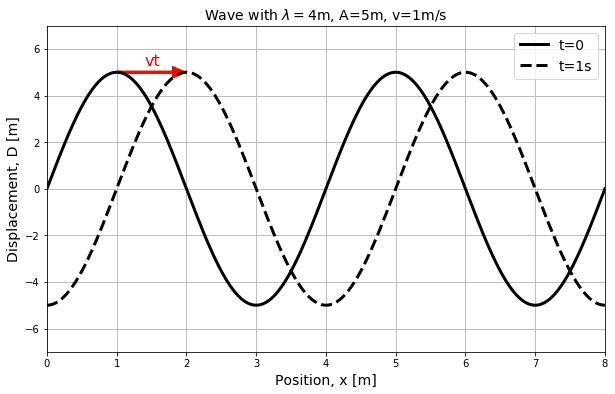
\includegraphics[width=0.7\linewidth]{files/sinewave-ada62bf73e73052cf695ebf0d37a8911.png}
\caption[]{Displacement as a function of position for particles in a medium as a wave passes through. The dotted line shows the dipsplacement as a function of time ${\rm 1/s}$ after the solid line, and corresponds to a wave travelling towards the right.}
\label{fig:waves:sinewave}
\end{figure}

The displacement, $D$, of each point at position, $x$, in the medium is shown on the vertical axis of Figure~\ref{fig:waves:sinewave}. The solid black line corresponds to a snapshot of the wave at time $t=0$. The wave has an amplitude, $A=5 {\rm m}$, a velocity, $v=1 {\rm m/s}$, and a wavelength, $\lambda=4 {\rm m}$. The dotted line corresponds to a snapshot of the wave one second later, at $t=1 {\rm s}$, when the wave has moved to the right by a distance $vt=1 {\rm m}$.

It is important to note that Figure~\ref{fig:waves:sinewave} is not restricted to describing transverse waves, even if the illustration suggests that the particles' displacements (vertical axis) are perpendicular to the direction of propagation of the wave (horizontal). The quantity, $D$, that is plotted on the vertical axis corresponds to the displacement of a particle from its equilibrium position. That displacement could correspond to the longitudinal displacement of a particle in a longitudinal wave.

At time $t=0$ (solid line), the displacement of each point in the medium, $D(x, t=0)$, as a function of their distance from the origin, $x$, can be described by a sine function:
\begin{equation}
D(x,t=0) = A\sin\left( \frac{2\pi}{\lambda}x \right)
\end{equation}
This corresponds to the displacement being 0 at the origin and at any position, $x$, that is a multiple of the wavelength, $\lambda$.

If the wave moves with velocity $v$ in the positive $x$ direction, then at time $t$, the sine function in Figure~\ref{fig:waves:sinewave} will have shifted to the right by an amount $vt$ (dotted line). The displacement of a point located at position $x$ at time $t$ will be the same as the displacement of the point at position $x -vt$ at time $t=0$. For example, in Figure~\ref{fig:waves:sinewave} the displacement of the point $x=2 {\rm m}$ at time $t=1 {\rm s}$ is the same as the displacement of the point at position $x -vt=1 {\rm m}$ at $t=0$.

We can state this condition as:
\begin{equation}
D(x,t) = D(x-vt, t=0)
\end{equation}
That is, at some time $t$, the displacement of a point at position $x$ is found by finding the position of the point at $x -vt$ at $t=0$. We already have an equation to find the displacement of a point at $t=0$.  Using the above condition, we can modify \href{\#eq:waves:wavex}{} to write a function for the displacement of a point at position $x$ at time $t$:
\begin{equation}
D(x,t) = A\sin\left( \frac{2\pi}{\lambda}(x-vt) \right)
\end{equation}
Noting that $v/\lambda= 1/T$, we can write this as:
\begin{equation}
D(x,t) = A\sin\left( \frac{2\pi x}{\lambda}- \frac{2\pi t}{T} \right)
\end{equation}
In the above derivation, we assumed that at time $t=0$, the displacement at $x=0$ was $D(x=0, t=0)=0$. In general, the displacement could have any value at $x=0$ and $t=0$, so we can allow the wave to shift left or right by including a phase, $\phi$, which can be determined from the displacement at $x=0$ and $t=0$:
\begin{equation}
\boxed{D(x,t) = A\sin\left( \frac{2\pi x}{\lambda}- \frac{2\pi t}{T} + \phi \right)}
\end{equation}
where $\phi=0$ corresponds to the displacement being zero at $x=0$ and $t=0$.

\begin{framed}
\textbf{Checkpoint}\\
What is the value of the phase $\phi$ if the displacement of the point at $x=0$ is $D=A/2$ at time $t=0$?\}

\begin{enumerate}
\item $\pi/6$.
\item $\pi/4$.
\item $\pi/3$.
\item $\pi/2$.
\end{enumerate}

\begin{framed}
\textbf{Answer}\\
\begin{enumerate}
\item
\end{enumerate}
\end{framed}
\end{framed}

The equation above is written in terms of the wavelength, $\lambda$, and period, $T$, of the wave. Often, one uses the ``wave number'', $k$, and the ``angular frequency'', $\omega$, to describe the wave. These are defined as:
\begin{equation}
k &= \frac{2\pi}{\lambda}\\
\omega &= \frac{2\pi}{T}
\end{equation}
Using the wave number and the angular frequency removes the factors of $2\pi$ in the expression for $D(x,t)$, which can now be written as:
\begin{equation}
\boxed{D(x,t) = A\sin\left( kx -\omega t + \phi \right)}
\end{equation}
It is important to note that the wave number, $k$, has no relation to the spring constant that we used for springs.

Using (\ref{eq:waves:speed}), we can also relate the wave number and angular frequency to the speed of the wave:
\begin{equation}
v = \frac{\lambda}{T}=\frac{\frac{2\pi}{k}}{\frac{2\pi}{\omega}}=\frac{\omega}{k}
\end{equation}

\paragraph{The wave equation}\label{sec:waves:waveequation}

In Section~\ref{chapter:simpleharmonicmotion}, we saw that any physical system whose position, $x$, satisfies the following equation:
\begin{equation}
\frac{d^2x}{dt^2}=-\omega^2 x
\end{equation}
will undergo simple harmonic motion with angular frequency $\omega$, and that $x(t)$ can be modelled as:
\begin{equation}
x(t) = A\cos(\omega t + \phi)
\end{equation}

Similarly, any system, where the displacement of a particle as a function of position and time, $D(x,t)$, satisfies the following equation:
\begin{equation}
\frac{\partial^2D}{\partial x^2}=\frac{1}{v^2}\frac{\partial^2D}{\partial t^2}
\end{equation}
is described by a wave that propagates with a speed $v$. The equation above is called the ``one-dimensional wave equation'' and would be obtained from modelling the dynamics of the system, just as the equation of motion for a simple harmonic oscillator can be obtained from Newton's Second Law. For the harmonic oscillator, the properties of the system (e.g. mass and spring constant) determine the angular frequency, $\omega$. For a wave, the properties of the medium determine the speed of the wave, $v$.

We use partial derivatives in the wave equation instead of total derivatives because $D(x,t)$ is multi-variate. A possible solution to the one-dimensional wave equation is:
\begin{equation}
D(x,t) = A\sin\left( kx -\omega t + \phi \right)
\end{equation}
which is the function that we used in the previous section to describe a sine wave.

Furthermore, if multiple solutions to the wave equation, $D_1(x,t)$, $D_2(x,t)$, etc, exist, then any linear combination, $D(x,t)$, of the solutions will also be a solution to the wave equation:
\begin{equation}
D(x,t) = a_1D_1(x,t)+a_2D_2(x,t)+a_3D_3(x,t)+\dots
\end{equation}
This last property is called ``the superposition principle'', and is the result of the wave equation being linear in $D$ (it does not depend on $D^2$, for example). It is easy to check, for example, that if $D_1(x,t)$ and $D_2(x,t)$ satisfy the wave equation, so does their sum.

In three dimensions, the displacement of a particle in the medium depends on its three spatial coordinates, $D(x,y,z,t)$, and the wave equation in Cartesian coordinates is given by:
\begin{equation}
\frac{\partial^2D}{\partial x^2}+\frac{\partial^2D}{\partial y^2}+\frac{\partial^2D}{\partial z^2}&=\frac{1}{v^2}\frac{\partial^2D}{\partial t^2}\\
\end{equation}
There are many functions that can satisfy this equation, and the best choice will depend on the physical system being modelled and the properties of the wave that one wishes to describe.

\subsubsection{Waves on a rope}

In this section, we model the motion of transverse waves on a rope, as this provides insight into many properties of waves that extend to waves propagating in other media.

\paragraph{A pulse on a rope}

We start by modelling how a single pulse propagates down a horizontal rope that is under a tension, $F_T$\footnote{We do not use $T$ for tension, so as to not confuse with the period of a wave.}. A wave is generally considered to be a regular series of alternating upwards and downwards pulses propagating down the rope. Modelling the propagation of a pulse is thus equivalent to modelling the propagation of a wave. Figure~\ref{fig:waves:pulse} shows how one can generate a pulse in a taught horizontal rope by raising (and then lowering) one end of the rope.

\begin{figure}[!htbp]
\centering
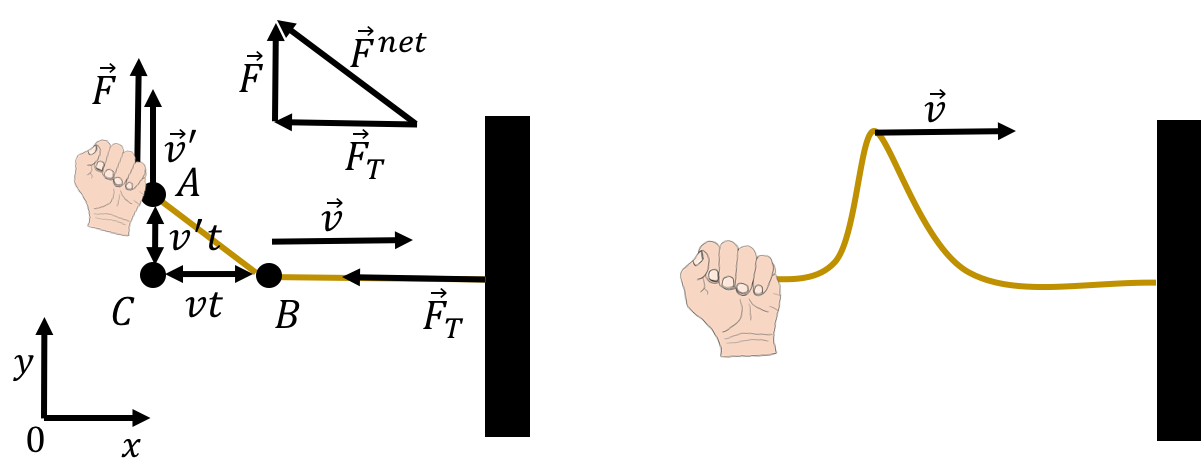
\includegraphics[width=0.8\linewidth]{files/pulse-5b40f374a8842266c668cb8b3a29c68d.png}
\caption[]{(Left:) Pulling upwards and then downwards on a horizontal rope causes a pulse to form and propagate. After a short period of time, a pulse is seen propagating down the rope (right).}
\label{fig:waves:pulse}
\end{figure}

We can model the propagation speed of the pulse by considering the speed, $v$, of point $B$ that is shown in the left panel of Figure~\ref{fig:waves:pulse}. Note that point $B$ is not a particle of the rope, and is, instead, the location of the ``front'' of the disturbance that the pulse causes on the rope. We model the rope as being under a horizontal force of tension, $\vec F_T$, and the pulse is started by exerting a vertical force, $\vec F$, to move the end (point $A$) of the rope upwards with a speed, $v'$. Thus, by pulling upwards on the rope with a force, $\vec F$, at a speed $v'$, we can start a disturbance in the rope that will propagate with speed $v$.

In a short amount of time, $t$, the point $A$ on the rope will have moved up by a distance $v't$, whereas point $B$ will have moved to the right by a distance $vt$. If $t$ is small enough, we can consider the points $A$, $B$, and $C$ to form the corners of a triangle. That triangle is similar to the triangle that is made by vectorially summing the applied force $\vec F$ and the tension $\vec F_T$, as shown in the top left of Figure~\ref{fig:waves:pulse}. In this case, we mean the geometry term ``similar'', which describes two triangles which have the same angles. We can thus write:
\begin{equation}
\frac{F}{F_T}&=\frac{v't}{vt}=\frac{v'}{v}\\
\therefore F&= F_T \frac{v'}{v}
\end{equation}
Consider the section of rope with length $vt$ that we have raised by applying that force (we assume that the distance $AB$ is approximately equal to the distance $BC$). If the rope has a mass per unit length $\mu$, then the mass of the rope element that was raised (between points $A$ and $B$) has a mass, $m$, given by:
\begin{equation}
m = \mu vt
\end{equation}
The vertical component of the momentum of that section of rope, with vertical speed given by $v'$, is thus:
\begin{equation}
p = mv' = \mu vt v'
\end{equation}
If the vertical force, $\vec F$, was exerted for a length of time, $t$, on the mass element, it will give it a vertical impulse, $Ft$, equal to the change in the vertical momentum of the mass element:
\begin{equation}
Ft &= \Delta p \\
Ft &= \mu vt v'\\
\therefore F &= \mu v v'
\end{equation}
We can equate this expression for $F$ with that obtained from the similar triangles to obtain an expression for the speed, $v$, of the pulse:
\begin{equation}
\mu v v' &= F_T \frac{v'}{v}\\
\therefore v&= \sqrt{\frac{F_T}{\mu}}
\end{equation}
The speed of a pulse (and wave) propagating through a rope with linear mass density, $\mu$, under a tension, $F_T$, is given by:
\begin{equation}
\boxed{v= \sqrt{\frac{F_T}{\mu}}}
\end{equation}
If the tension in the rope is higher, the pulse will propagate faster. If the linear mass density of the rope is higher, then the pulse will propagate slower.

\paragraph{Reflection and transmission}\label{subsec:waves:reflection}

In this section, we examine what happens when a pulse travelling down a rope arrives at the end of the rope. First, consider the case illustrated in Figure~\ref{fig:waves:reflectionfixed} where the end of the rope is fixed to a wall.

\begin{figure}[!htbp]
\centering
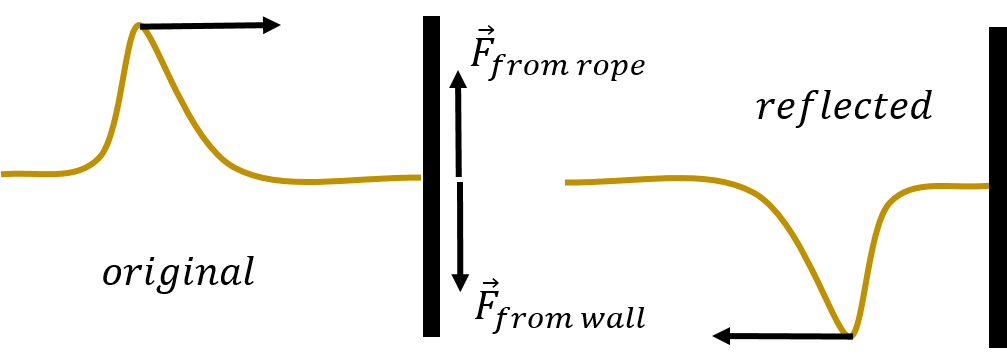
\includegraphics[width=0.7\linewidth]{files/reflectionfixed-d7f14aaeb523e5a462f490a2ba33146d.png}
\caption[]{When the end of the rope is held fixed, the reflected pulse will be inverted.}
\label{fig:waves:reflectionfixed}
\end{figure}

When the pulse arrives at the wall, the rope will exert an upwards force on the wall, $\vec F_{from\; rope}$. By Newton's Third Law, the wall will then exert a downwards force on the rope, $\vec F_{from\; wall}$. The downwards force exerted on the rope will cause a downwards pulse to form, and the reflected pulse will be inverted compared to the initial pulse that arrived at the wall.

Now, consider the case when the end of the rope has a ring attached to it, so that it can slide freely up and down a post, as illustrated in Figure~\ref{fig:waves:reflectionfree}.

\begin{figure}[!htbp]
\centering
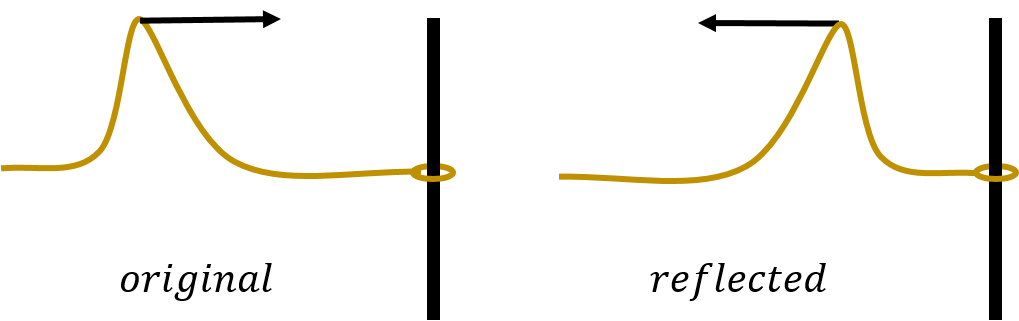
\includegraphics[width=0.7\linewidth]{files/reflectionfree-24178e7e12fb7cac8d1acb9146619fb7.png}
\caption[]{When the end of the rope is free, the reflected pulse will be upright.}
\label{fig:waves:reflectionfree}
\end{figure}

In this case, the end of the rope will move up as the pulse arrives, which will then create a reflected pulse that is in the same orientation as the incoming pulse.

Finally, consider a pulse that propagates down a rope of mass per unit length $\mu_1$ that is tied to a second rope with mass per unit length $\mu_2$, which have the same tension. When the pulse arrives at the interface between the two media (the two ropes), part of the pulse will be reflected back, and part will be transmitted into the second medium (Figure~\ref{fig:waves:transmission}).

\begin{figure}[!htbp]
\centering
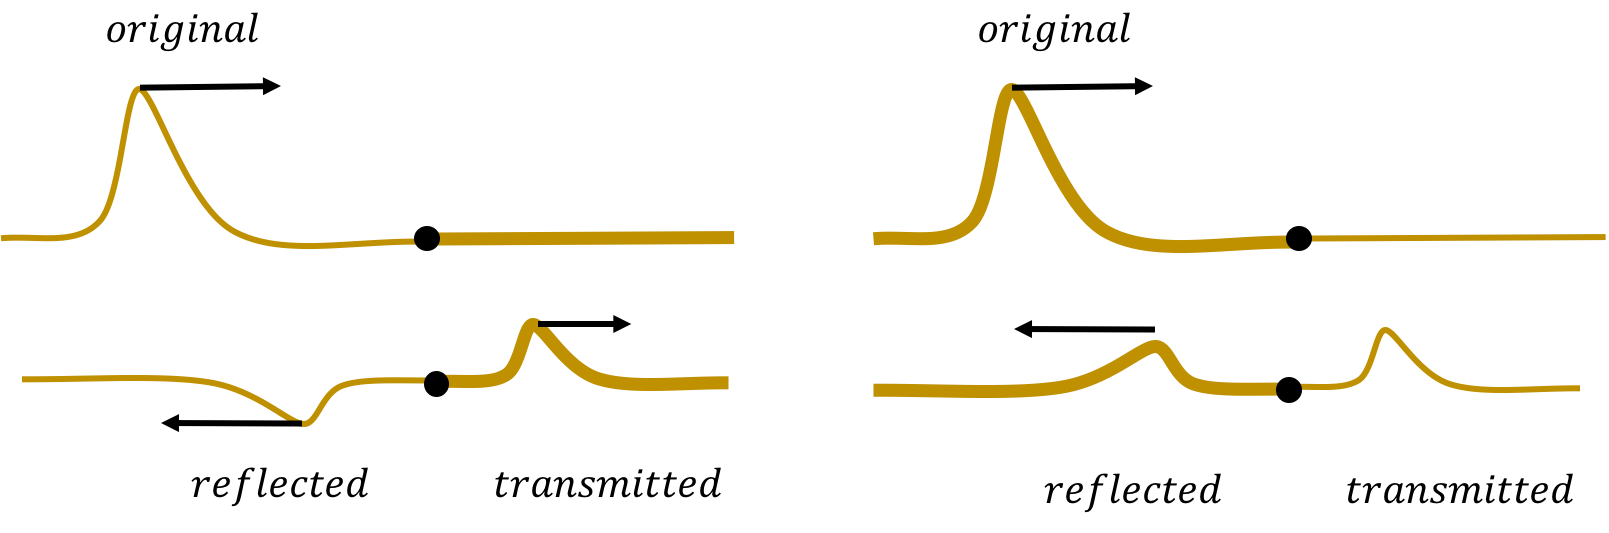
\includegraphics[width=0.8\linewidth]{files/transmission-21e5709e7a17f00aa0a9ec4a22f01bb3.png}
\caption[]{A pulse can be both reflected and transmitted as it changes medium. Left panel: The pulse is transmitted from a lighter rope to a heavier rope. Right panel: The pulse is transmitted from a heavier rope to a lighter rope}
\label{fig:waves:transmission}
\end{figure}

By considering the boundary conditions, one can derive the coefficient of reflection, $R$ (see Section~\ref{sec:problemswaves} for the derivation). This coefficient is the ratio of the amplitude of the reflected pulse to the amplitude of initial pulse. The ratio is found to be:
\begin{equation}
R=\frac{\sqrt{\mu_1}-\sqrt{\mu_2}}{\sqrt{\mu_1}+\sqrt{\mu_2}}
\end{equation}
When the pulse moves from a lighter rope to a heavier rope ($\mu_1<\mu_2$), the reflected pulse will be inverted ($R<0$). When the pulse moves from a heavier rope to a lighter rope ($\mu_1>\mu_2$), the reflected pulse will stay upright ($R>0$).

When the end of the rope is fixed to a wall (as in Figure~\ref{fig:waves:reflectionfixed}), this represents a limiting case in which the linear mass density of the second material approaches infinity ($\mu_2 \rightarrow \infty$):
\begin{equation}
R=\lim_{\mu_2\to \infty}\frac{\sqrt{\mu_1}-\sqrt{\mu_2}}{\sqrt{\mu_1}+\sqrt{\mu_2}}=\frac{-\sqrt{\mu_2}}{\sqrt{\mu_2}}=-1
\end{equation}
which means that the amplitude of the reflected pulse will have the same magnitude as the initial pulse but will be in the opposite direction. When the end of the rope is free (Figure~\ref{fig:waves:reflectionfree}), this represents another limiting case, where $\mu_2\rightarrow 0$:
\begin{equation}
R=\lim_{\mu_2\to 0}\frac{\sqrt{\mu_1}-\sqrt{\mu_2}}{\sqrt{\mu_1}+\sqrt{\mu_2}}=\frac{\sqrt{\mu_1}}{\sqrt{\mu_1}}=1
\end{equation}
which means that the amplitude of the reflected pulse will be in the same direction  and have the same amplitude as the initial pulse.

\begin{framed}
\textbf{Checkpoint}\\
A wave propagates from a light rope to a heavier rope that is attached to the light rope (as the pulse illustrated in Figure~\ref{fig:waves:transmission}). What can you say about the wavelength of the wave on either side of the interface?

\begin{enumerate}
\item It is the same in both sections of rope.
\item The wavelength in the heavy section of rope is longer.
\item The wavelength in the light section of rope is longer.
\end{enumerate}

\begin{framed}
\textbf{Answer}\\
\begin{enumerate}[resume]
\item
\end{enumerate}
\end{framed}
\end{framed}

\paragraph{The wave equation for a rope}

In this section, we show how to use Newton's Second Law to derive the wave equation for transverse waves travelling down a rope with linear mass density, $\mu$, under a tension, $F_T$. Consider a small section of the rope, with mass $dm$, and length $dx$, as a wave passes through that section of the rope, as illustrated in Figure~\ref{fig:waves:weqn}.

\begin{figure}[!htbp]
\centering
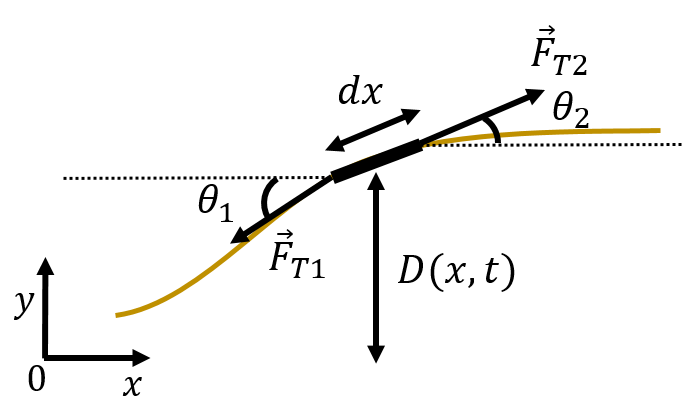
\includegraphics[width=0.55\linewidth]{files/weqn-7b90038e7759d28c72dec85d39be882d.png}
\caption[]{A small section of rope under tension as a wave passes through.}
\label{fig:waves:weqn}
\end{figure}

We assume that the weight of the mass element is negligible compared to the force of tension that is in the rope. Thus, the only forces exerted on the mass element are those from the tension in the rope, pulling on the mass element from each side, with forces, $\vec F_{T1}$ and $\vec F_{T2}$. In general, the forces from tension on either side of the mass element will have different directions and make different angles, $\theta$, with the horizontal, although their magnitude is the same. Let $D(x,t)$ be the vertical displacement of the mass element located at position $x$. We can write the $y$ (vertical) component of Newton's Second Law for the mass element, $dm$, as:
\begin{equation}
\sum F_y = F_{T2y} - F_{T1y} &= (dm)a_y\\
F_T\sin\theta_2 - F_T\sin\theta_1 &= dm \frac{\partial ^2D}{\partial t^2}\\
F_T(\sin\theta_2 - \sin\theta_1) &= dm \frac{\partial ^2D}{\partial t^2}
\end{equation}
where we used the fact that the force of tension has a magnitude, $F_T$, on either side of the mass element, and that the acceleration of the mass in the vertical direction is the second time-derivative of $D(x,t)$, since for a transverse wave, this corresponds to the $y$ position of a particle. We now make the small angle approximation:
\begin{equation}
\sin\theta\approx \tan\theta = \frac{\partial D}{\partial x}
\end{equation}
in which the sine of the angle is approximately equal to the tangent of the angle, which is equal to the slope of the rope. Applying this approximation to Newton's Second Law:
\begin{equation}
F_T\left(\frac{\partial D}{\partial x}\Bigr|_{right} - \frac{\partial D}{\partial x}\Bigr|_{left}\right) &= dm \frac{\partial ^2D}{\partial t^2}
\end{equation}
where we indicated that the term in parentheses is the difference in the slope of the rope between the right side and the left side of the mass element. If the rope has linear mass density, $\mu$, then the mass of the rope element can be expressed in terms of its length, $dx$:
\begin{equation}
dm = \mu dx
\end{equation}
Replacing $dm$ in the equation gives:
\begin{equation}
F_T\left(\frac{\partial D}{\partial x}\Bigr|_{right} - \frac{\partial D}{\partial x}\Bigr|_{left}\right) &= \mu dx \frac{\partial ^2D}{\partial t^2}\\
F_T\left(\frac{\frac{\partial D}{\partial x}\Bigr|_{right} - \frac{\partial D}{\partial x}\Bigr|_{left}}{dx}\right) &= \mu \frac{\partial ^2D}{\partial t^2}
\end{equation}
The term in parentheses is the difference in the first derivatives of $D(x,t)$ with respect to $x$, divided by the distance, $dx$, between which those derivatives are evaluated. This is precisely the definition of the second derivative with respect to $x$, so we can write:
\begin{equation}
F_T \frac{\partial ^2D}{\partial x^2} &= \mu \frac{\partial ^2D}{\partial t^2}\\
\therefore \frac{\partial ^2D}{\partial x^2} &= \frac{\mu}{F_T} \frac{\partial ^2D}{\partial t^2}\\
\end{equation}
which is precisely the wave equation:
\begin{equation}
\frac{\partial ^2D}{\partial x^2} &= \frac{1}{v^2} \frac{\partial ^2D}{\partial t^2}\\
\end{equation}
with speed:
\begin{equation}
v&= \sqrt{\frac{F_T}{\mu}}
\end{equation}
as we found earlier. Thus, we find that the speed of the propagation of the wave is related to the dynamics of modelling the system, and is not related to the wave itself.

\subsubsection{The speed of a wave}

In the previous section we found that the speed of a transverse wave in a rope is related to the ratio of the tension in the rope to the linear mass density of the rope:
\begin{equation}
v&= \sqrt{\frac{F_T}{\mu}}
\end{equation}
The speed of a wave in any medium is usually given by a ratio, where the numerator is a measure of how easy it is to deform the medium, and the denominator is measure of the inertia of the medium. For a rope, the tension is a measure of how stiff the rope is. A higher tension makes it more difficult to disturb the rope from equilibrium and it will ``snap back'' faster when disturbed, so the pulse will propagate faster. The heavier the rope, the harder it will be for the disturbance to propagate as the rope has more inertia, which will slow down the pulse.

The only way that a wave can propagate through a medium is if that medium can be deformed and the particles in the medium can be displaced from their equilibrium position, much like simple harmonic oscillators. The wave will propagate faster if those oscillators have a stiff spring constant and there is a strong force trying to restore them to equilibrium. However, if those oscillators have a large inertia, even with a large restoring force, they will accelerate back to their equilibrium with a smaller acceleration.

In general, the speed of a wave is given by:
\begin{equation}
v=\sqrt{\frac{\text{Stiffness of medium}}{\text{Inertia of medium}}}
\end{equation}
For example, the speed of longitudinal pressure waves in a solid is given by:
\begin{equation}
v=\sqrt{\frac{E}{\rho}}
\end{equation}
where $E$ is the ``elastic (or Young's) modulus'' for the material, and $\rho$ is the density of the material. The elastic modulus of a solid is a measure of the material's resistance to being deformed when a force (or pressure) is exerted on it. The more easily it is deformed, the lower its elastic modulus will be.

For the propagation of longitudinal pressure waves through a fluid, the speed is given by:
\begin{equation}
v=\sqrt{\frac{B}{\rho}}
\end{equation}
where $B$ is the bulk modulus of the liquid, and $\rho$ its density.

\begin{framed}
\textbf{Checkpoint}\\
A wave will propagate faster through...

\begin{enumerate}
\item ice.
\item water.
\end{enumerate}

\begin{framed}
\textbf{Answer}\\
\begin{enumerate}
\item
\end{enumerate}
\end{framed}
\end{framed}

\subsubsection{Energy transported by a wave}

In this section, we examine how to model the energy that is transported by waves. Although no material moves along with a wave, mechanical energy can be transported by a wave, as evidenced by the damage caused by the waves from an earthquake.

\paragraph{A wave as being made of simple harmonic oscillators}

Consider a wave that is propagating through a medium. We can model the motion of one of the particles in the medium as if it were the motion of a simple harmonic oscillator\footnote{If the medium has a linear restoring force or if the amplitude of the oscillations is small.}. This is illustrated in Figure~\ref{fig:waves:sinewavetimeshm}, which shows the displacement \textbf{as a function of time} for a point in the medium located at the origin when a wave passes through that point. The displacement of that point, at $x=0$, if we choose $\phi=0$, is given by:
\begin{equation}
D(x=0,t) = A\sin(-\omega t)
\end{equation}
\begin{figure}[!htbp]
\centering
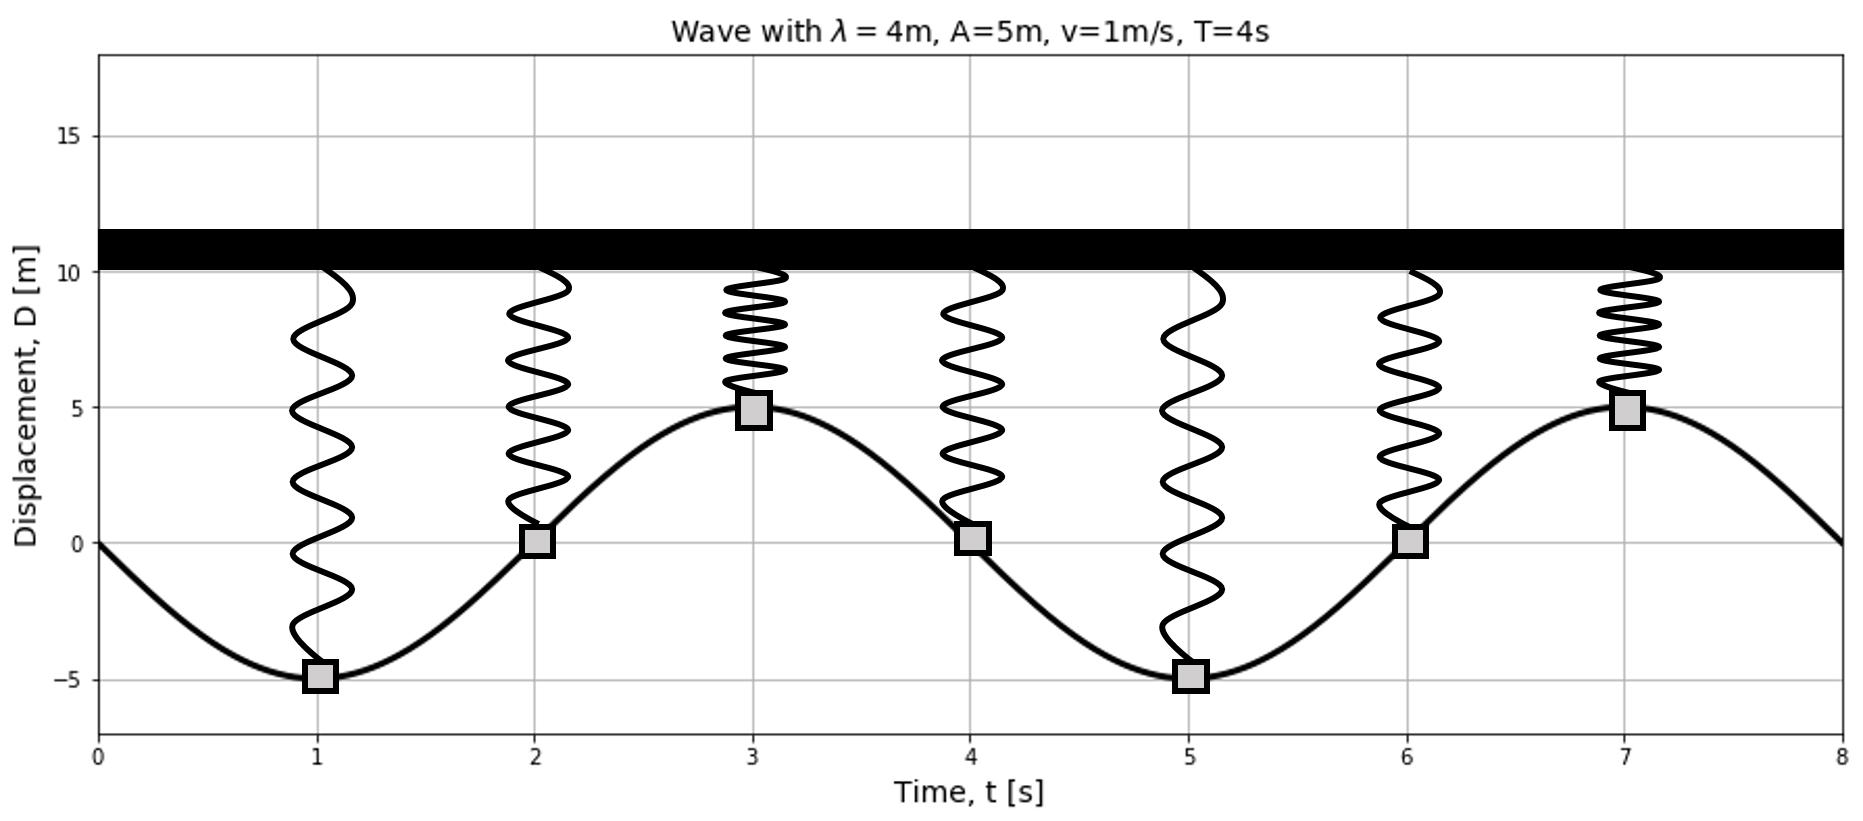
\includegraphics[width=0.8\linewidth]{files/sinewavetimeshm-17f892d05b9c06df3c5af67634ed5e59.png}
\caption[]{The displacement as a function of time for one particle in the medium (at $x=0$) is identical to the motion of a simple harmonic oscillator.}
\label{fig:waves:sinewavetimeshm}
\end{figure}

The displacement of the particle in the medium is described by the same equation as the position of a simple harmonic oscillator, with the same angular frequency $\omega$, as that of the wave.

We can also view a snapshot of the wave in time, and model the \textbf{different} points in the medium as different oscillators that all have different displacements. This is shown in Figure~\ref{fig:waves:sinewavepositionshm}.

\begin{figure}[!htbp]
\centering
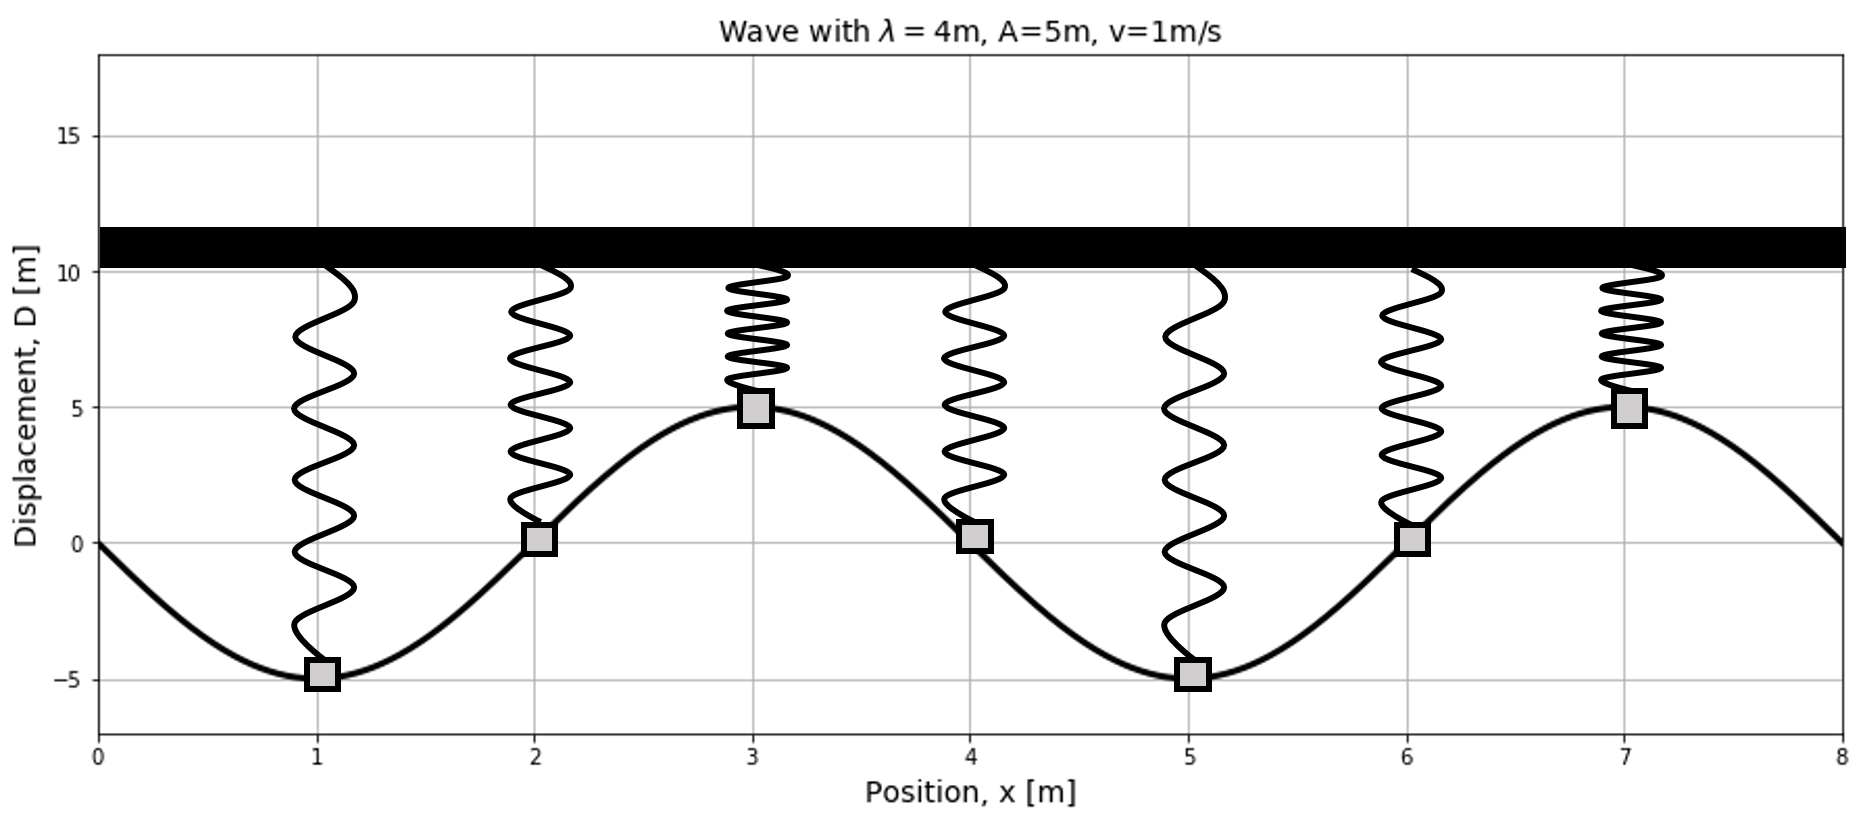
\includegraphics[width=0.8\linewidth]{files/sinewavepositionshm-741b248e606f6bc4de96e5802f76595e.png}
\caption[]{The displacement as a function of position for different points in a medium. Each point in the medium can be modelled as a simple harmonic oscillator.}
\label{fig:waves:sinewavepositionshm}
\end{figure}

\paragraph{Energy transported in a one dimensional wave}

In this section, we show how to describe the energy transported by a one-dimensional wave along a rope. We model each particle in the rope through which the wave propagates as a small simple harmonic oscillator with mass $m$, attached to a spring with an effective spring constant, $k_s$\footnote{We use $k_s$ for the spring constant, to distinguish it from $k$, the wave number.}.

Of course, there is no actual spring, but we can still determine an effective spring constant, $k_s$, from the angular frequency:
\begin{equation}
\omega &= \sqrt{\frac{k_s}{m}}\\
\therefore k_s &= \omega^2 m
\end{equation}
which corresponds to the spring constant that would give the correct angular frequency for the particle of mass $m$.

The total mechanical energy of one oscillator, $E_m$, can be evaluated when the oscillator is at its maximal displacement, $A$, from its equilibrium, where its kinetic energy is zero:
\begin{equation}
E_m = \frac{1}{2}k_s A^2 = \frac{1}{2}\omega^2 m A^2
\end{equation}

If the rope is infinitely long, and carries a continuous wave, it will have an infinite amount of energy, as it will correspond to an infinite number of oscillators. Instead, let us calculate how much energy, $E_\lambda$, is stored in the wave over one wavelength, $\lambda$. To do so, we need to evaluate how many effective oscillators are contained in the rope, over a distance $\lambda$, so that we can sum all of their energies together to obtain the energy stored in one wavelength:
\begin{equation}
E_\lambda = \sum \frac{1}{2}\omega^2 m A^2
\end{equation}
where the sum is over the number of oscillators in one wavelength. Of course, the rope is not actually made of oscillators, but we can model each section of rope of length $dx$ has being an oscillator of mass $dm=\mu dx$, where $\mu$ is the linear mass density of the rope. The sum (integral) of the energy of the oscillators over one wavelength can thus be written as:
\begin{equation}
E_\lambda = \int_0^\lambda \frac{1}{2}\omega^2 \mu A^2 dx =  \frac{1}{2}\omega^2 \mu A^2 \lambda
\end{equation}
The energy stored in one wavelength is not a very useful property of a wave, since the total energy in the wave depends on the length of the wave. We can describe the rate at which energy is transmitted by the wave (its power), since we know how long, $T$, it will take the wave to travel one wavelength, and we just determined how much energy is stored in one wavelength. The average power with which energy is transported by a wave is given by:
\begin{equation}
P = \frac{E_\lambda}{T} = \frac{\frac{1}{2}\omega^2 \mu A^2 \lambda}{T}=\frac{1}{2}\omega^2 \mu A^2 v
\end{equation}
where $T$ is the period of the wave, and $v=\lambda/T$ is the speed of the wave. The power transmitted by a wave on a rope is thus given by:
\begin{equation}
\boxed{P=\frac{1}{2}\omega^2 \mu A^2 v}
\end{equation}
We can see that the power transmitted by a wave goes as the amplitude, $A$, of the wave squared. It thus takes four times more energy to double the amplitude of waves that are sent down a rope.

\paragraph{Energy transported in a spherical, three-dimensional, wave}

In this section, we show how to model the rate at which energy is transported in spherical three-dimensional waves, such as the sound waves that are generated when you clap your hands. A spherical sound wave is a pressure disturbance in the air that propagates spherically outwards from a point of emission. We can think of thin spherical shells containing air that expand and contract about their equilibrium position as the wave moves through the shells. The motion of each shell is similar to that of a simple harmonic oscillator of mass $dm$, where $dm$ is the mass of air in the oscillating shell.

\begin{figure}[!htbp]
\centering
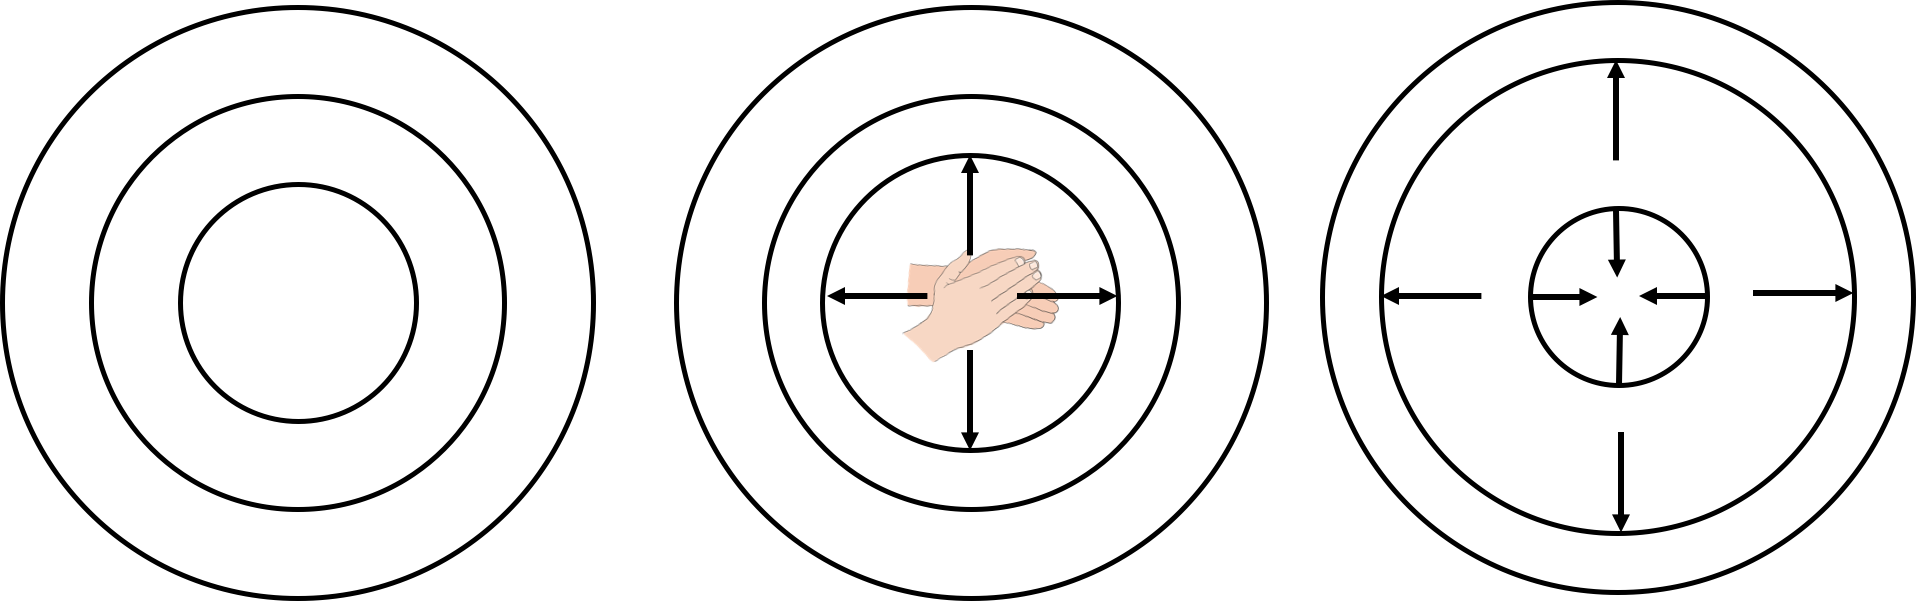
\includegraphics[width=0.9\linewidth]{files/sphericalwave-bd8937037f04d3c07c03e3fda3b6640b.png}
\caption[]{Left: We divide the air into thin spherical shells. Here we represent three shells (the black circles). Center: When you clap, the innermost shell is given energy and expands. Right: Energy is transferred to the next shell, which expands as the first shell contracts. This is how the wave propagates outwards. When the shells are closer together, the air molecules are closer together and exert a pressure that tries to expand the shell.}
\label{fig:waves:sphericalwave}
\end{figure}

Consider a shell at a radial position, $r$, from the source, with thickness $dr$, and mass $dm$:

\begin{figure}[!htbp]
\centering
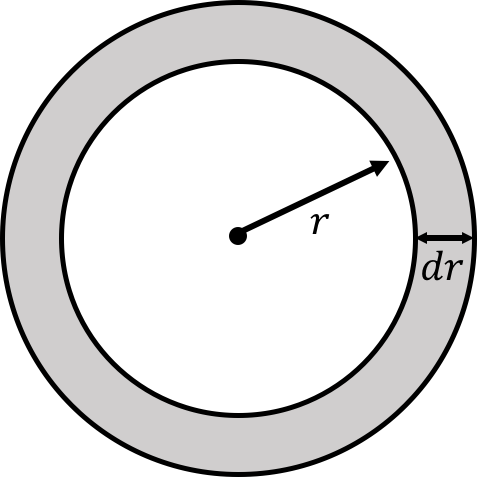
\includegraphics[width=0.3\linewidth]{files/sphericalshell-147d744283ba3a950fc86a57c3064a38.png}
\caption[]{A spherical shell at radial position $r$ with thickness $dr$}
\label{fig:waves:sphericalshell}
\end{figure}

If the medium has a density, $\rho$, then the mass of the shell is given by:
\begin{equation}
dm = \rho dV = \rho 4\pi r^2 dr
\end{equation}
where $dV = 4\pi r^2 dr$ is the volume of the shell. Again, if we model each shell as a simple harmonic oscillator with mass $dm$, then the energy, $dE$, stored in that oscillating shell is given by:
\begin{equation}
dE = \frac{1}{2}k_s A^2 =  \frac{1}{2}\omega^2 dm A^2 = \frac{1}{2}\omega^2 A^2 \rho 4\pi r^2 dr=2\pi\rho  \omega^2 A^2  r^2 dr
\end{equation}
where $\omega$ is the angular frequency of the wave, and $A$ is the amplitude of the wave. We expressed the effective spring constant, $k_s$, in terms of the angular frequency of the simple harmonic oscillator and its mass, as we did in the previous section. It now makes less sense to determine the energy that is stored in one wavelength of the wave because the energy, $dE$, stored in one shell depends on the location, $r$, of that shell. This was not the case for a one-dimensional wave, where the energy stored in one oscillator did not depend on the position of that oscillator.

The rate at which energy is transported by the wave is given by:
\begin{equation}
P = \frac{dE}{dt}
\end{equation}
We can use the Chain Rule to change this into a derivative over $r$:
\begin{equation}
P = \frac{dE}{dr}\frac{dr}{dt}=\frac{dE}{dr}v
\end{equation}
where $\frac{dr}{dt}=v$ is the speed of the wave (the rate of change of the radius of a shell). The power transmitted by the spherical wave is thus given by:
\begin{equation}
P &=\frac{dE}{dr}v =2\pi\rho  \omega^2 A^2  r^2 v
\end{equation}
where the power appears to depends on how far you are from the source ($r$).

Suppose that you have a $50 {\rm W}$ speaker emitting sound; each radial shell emanating from the speaker must transport energy at a rate of $50 {\rm W}$. This is simply a statement that the energy radiated by the speaker has to move from one shell to the next and be conserved. Since the power transported by a shell appears to depend on the radius of the shell, if the power transmitted by each shell is the same, then the amplitude of the wave in each shell must decrease, so that the power does not actually depend on the radius of the shell. In particular, for a spherical wave, the amplitude will decrease as a function of distance from the source:
\begin{equation}
P& = \text{constant}\\
\therefore A&=\frac{1}{r}\sqrt{\frac{P}{2\pi\rho \omega^2 v}}
\end{equation}
This is very different from the propagation of a one-dimensional wave, in which the amplitude does not change with distance. In practice, if there are energy losses due to, say, friction, then the amplitude of a one-dimensional wave would also decrease with distance from the source, but this is a different effect.

\begin{framed}
\textbf{Olivia's Thoughts}\\
Here's a slightly different way to think about why the amplitude of the wave decreases as you get further from the source. When a spherical wave travels outwards, energy is passed from one shell to the next. The outer shells are bigger than the inner shells, and so they will contain more particles. Because of conservation of energy, when the energy is transferred from one shell to the next, the total energy stays the same. In the outer shells, the energy must be shared between a greater number of particles, so each particle gets less energy, and therefore oscillates with a smaller amplitude than the particles in the previous shell did.

To remember this, imagine the shells in Figure~\ref{fig:waves:sphericalwave} are circles of kids standing side by side. The innermost circle has 10 kids and the outermost circle has 100 kids. If you have 100 candies, and you give them to the kids in the innermost circle, each will get 10 so they will get really hyper and start jumping around a lot. If you instead give the 100 candies to the kids in the outermost circle, each will only get one. The kids will only get a little bit hyper and jump around less.
\end{framed}

The ``intensity of a wave'', $I$, is defined as the power per unit area that is transmitted by the wave. For a spherical wave front at radial position $r$, with area $4\pi r^2$, the intensity of the wave is defined as:
\begin{equation}
I = \frac{P}{4\pi r^2} = \frac{1}{2}\rho  \omega^2 A^2 v
\end{equation}

Usually, the intensity of a wave is something that you can measure, as it corresponds to the power delivered into some measuring device with a known surface area. For example, we cannot directly measure the total power that is transported by the waves from an earthquake, as we would need an instrument that could encompass the entire resulting wave. Instead, we can measure the intensity of waves from the earthquake by measuring how much power is delivered into some instrument with a known surface area. By knowing our distance from the earthquake, we could then determine the total power output of the earthquake.

The intensity is a measure of how much energy is delivered per unit area by a wave and goes down as the square of the distance from the source (since $A\propto 1/r$). If the source of the wave is an earthquake, then your house will have four times less damage than your friend's, if your house is located only twice as far from the epicentre as your friend's. You will cause four times less damage to your ears if you move only twice as far away from the stage at a rock concert.

\subsubsection{Superposition of waves and interference}

In this section, we consider what happens when two (or more) different waves propagate in a medium and interfere with each other. The superposition principle states that if $D_1(x,t)$, $D_2(x,t)$, etc, are functions that satisfy the wave equation, then any linear combination of these functions, $D(x,t)$:
\begin{equation}
D(x,t) = a_1D_1(x,t)+a_2D_2(x,t)+a_3D_3(x,t)+\dots
\end{equation}
will also satisfy the wave equation.

Suppose that you hold one end of a rope and shake it with a specific frequency, creating waves that are described by:
\begin{equation}
D_1(x,t) = A_1\sin(k_1x-\omega_1t+\phi_1)
\end{equation}
Your friend, at the other end of the rope shakes the rope with a different frequency, creating waves that propagate in the opposite direction and that are described by:
\begin{equation}
D_2(x,t) = A_2\sin(k_2x+\omega_2t+\phi_2)
\end{equation}
The superposition principle states that the net displacement at any position $x$ at some time $t$ can be found by summing the displacement from the two waves together:
\begin{equation}
D(x,t) = A_1\sin(k_1x-\omega_1t+\phi_1) + A_2\sin(k_2x+\omega_2t+\phi_2)
\end{equation}

The superposition of waves is illustrated in Figure~\ref{fig:waves:superposition}, which shows three waves, and their resulting sum in the bottom most panel.

\begin{figure}[!htbp]
\centering
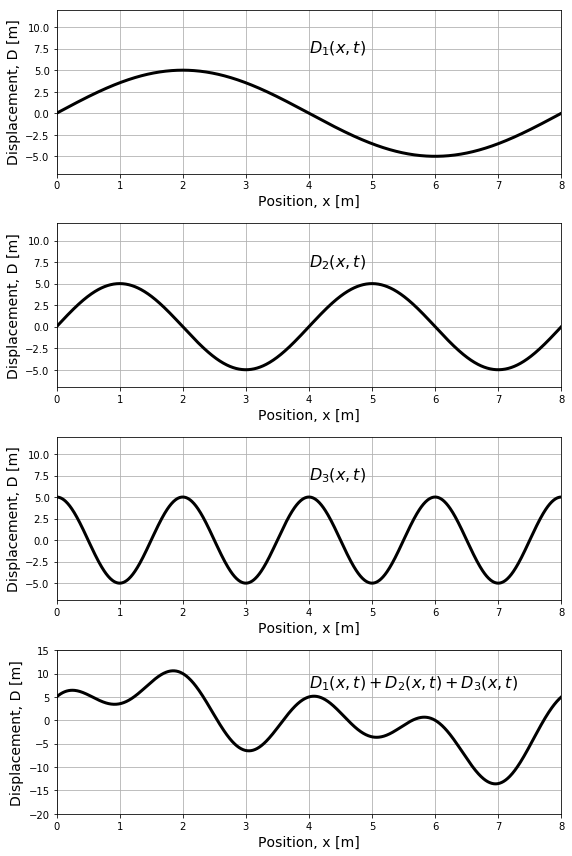
\includegraphics[width=0.7\linewidth]{files/superposition-77299987696f501413b72354db171fd4.png}
\caption[]{The superposition of three waves to create a resulting wave shown in the bottom panel. The waves are shown as the displacement as a function of position at a fixed instant in time.}
\label{fig:waves:superposition}
\end{figure}

The resulting wave is created by the ``interference'' of the three waves, and mathematically is simply a sum of the three individual waves at each position (and instant in time). The resulting wave in this example has a rather complicated shape, that is no longer described by a sine function. However, by the superposition principle, it is a valid solution to the wave equation\footnote{Fourier's Theorem states that any periodic function can be described as the linear combination of sine (or cosine) functions. This is the reason why we focused on using a sine function to describe a wave.}.

The individual waves in the top three panels of Figure~\ref{fig:waves:superposition} all have an amplitude of $5 {\rm m}$. The resulting wave, at some points (e.g. at $x=2 {\rm m}$), has an amplitude that is larger than any of the individual waves; we say that, at those positions, the individual waves have ``constructively interfered''. In other locations (e.g. at $x=6 {\rm m}$), the resulting wave has a smaller amplitude than the individual waves, and we say that the individual waves have ``destructively interfered''. The interference between waves can be observed easily on a water surface, for example by observing the constructive and destructive interference pattern of waves that originate from two pebbles being dropped at the same time a certain distance apart. Constructive interference between waves is also thought to be behind some reports of gigantic waves observed out at sea.

If two waves have the same wavelength and amplitude, it is possible for them to completely destructively interfere, resulting in no net wave. Similarly, they can also completely constructively interfere, resulting in a wave with a larger amplitude. Complete destructive and constructive interference are illustrated in the left and right panel of Figure~\ref{fig:waves:interference}, respectively.

\begin{figure}[!htbp]
\centering
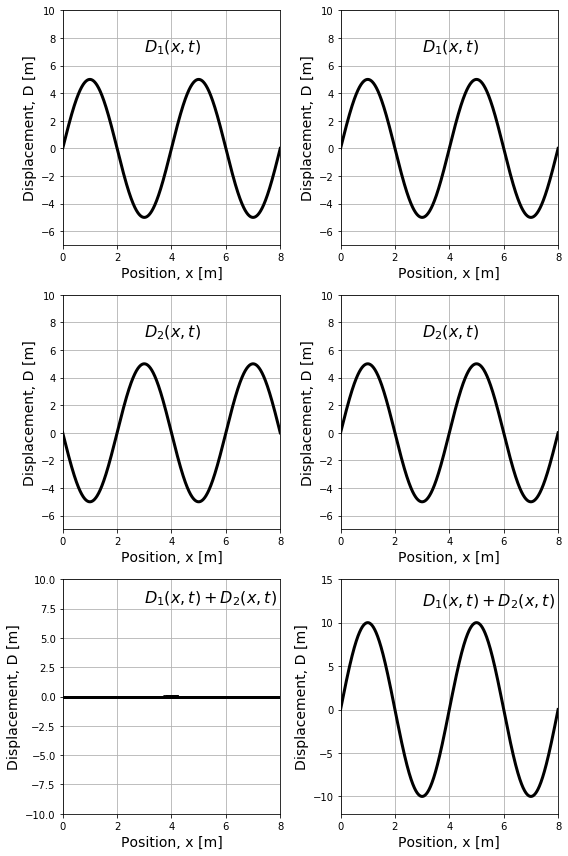
\includegraphics[width=0.7\linewidth]{files/interference-abb5ab7de5dbb86607a9e3c87ada0366.png}
\caption[]{Destructive (left) and constructive (right) interference of waves.}
\label{fig:waves:interference}
\end{figure}

\subsubsection{Standing waves}

As we saw in the last section, when waves have the same frequency, it is possible for them to interfere completely, either destructively or constructively. Waves of the same frequency that interfere can be generated by propagating waves along a string, as the reflected waves from the end of the string will have the same frequency as, and interfere with, the original waves. In general, the resulting wave will be quite complicated, but if you ``choose'' the frequency (or wavelength) of the generated waves precisely, then the waves will interfere and create a ``standing wave''. The standing wave is named this way because it does not appear to propagate along the string. Instead, each point on the string will oscillate with an amplitude that depends on where the point is located along on the string. In contrast, for a travelling wave, all of the points oscillate with the same amplitude.

Three standing waves of different frequencies (wavelengths) are illustrated in Figure~\ref{fig:waves:standing}.

\begin{figure}[!htbp]
\centering
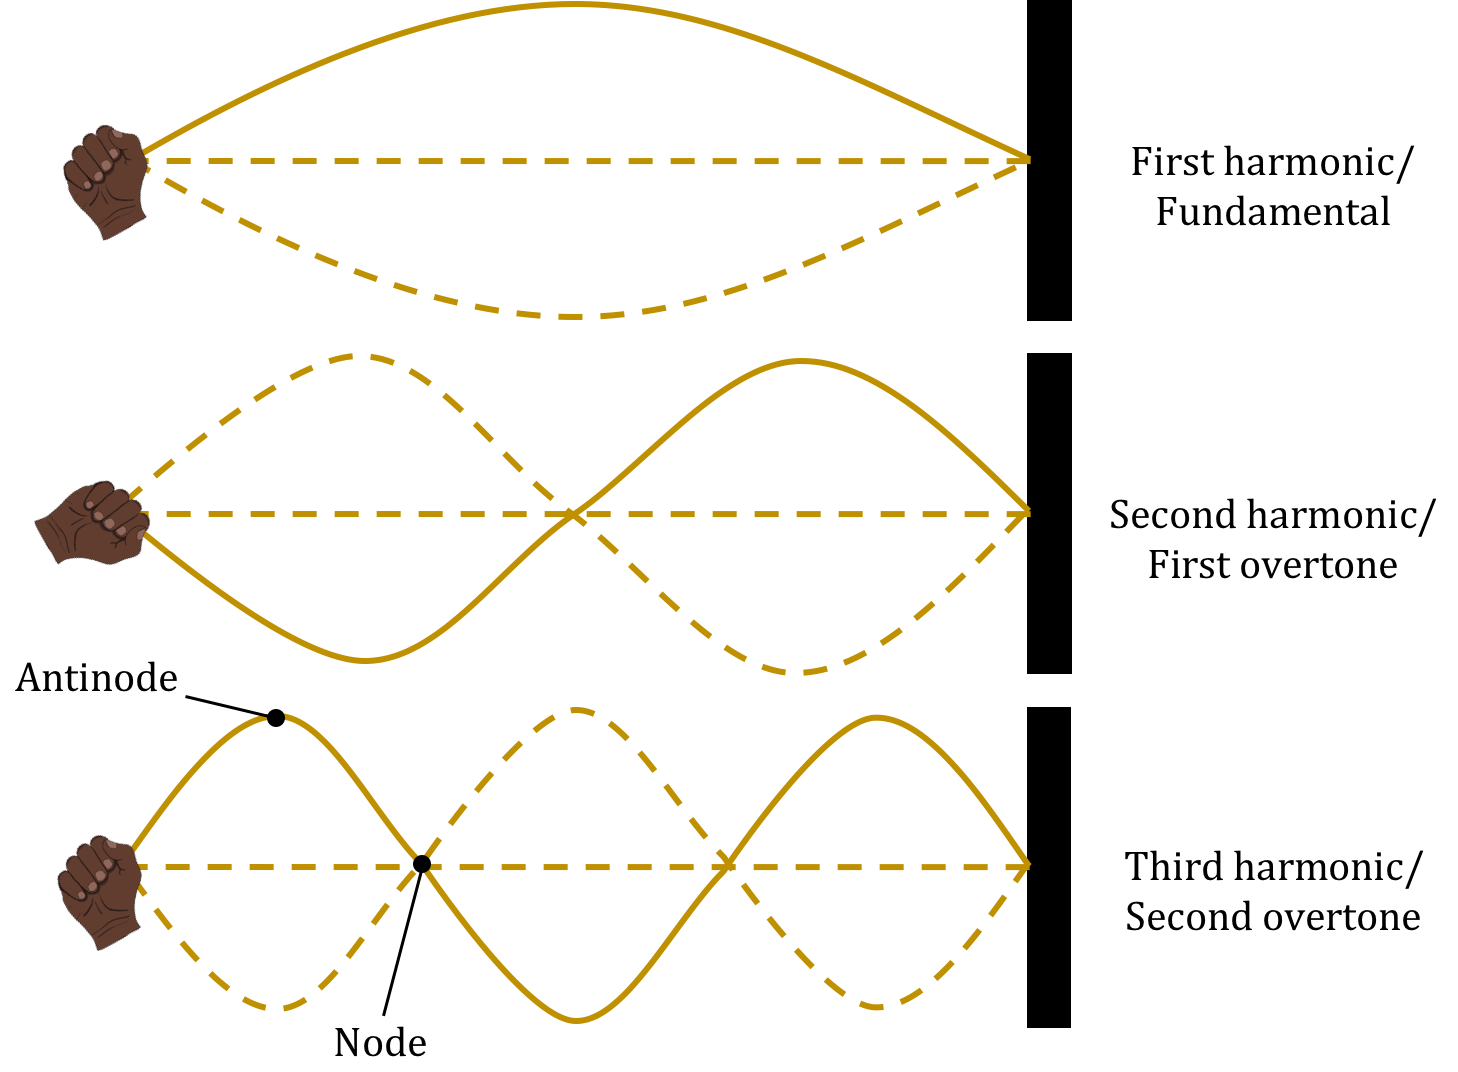
\includegraphics[width=0.7\linewidth]{files/standing-8a3bc3fb194afc707328d9f485a51d61.png}
\caption[]{The first three standing waves on a string.}
\label{fig:waves:standing}
\end{figure}

The solid line in each of the three panels corresponds to one particular snapshot of the standing wave at a particular instant in time. The dashed lines correspond to snapshots at different times. In particular, there is a time where the displacement of all points on the string is zero. Each point on the string vibrates with a different amplitude, which corresponds to the solid line (and the opposite dashed line). Certain points do not oscillate at all; these are called ``nodes''. The points at the end of the string are always nodes. Certain points vibrate with a maximal amplitude; these are called ``anti-nodes''.

In general, if you pluck a taught string (such as a guitar string), you will create a complicated wave, equivalent to many sine waves with different frequencies, that propagate outwards from the point where the string was plucked. Those sine waves will be reflected by the ends of the string and interfere with each other. Most of the waves will interfere in a complicated way and decay away. Those waves that have the correct frequency to create standing waves will persist on the string for a longer period of time. The string will eventually vibrate as a superposition of the fundamental frequency (the standing wave with one anti-node, also called the first harmonic), and the higher ``harmonics'' (those standing waves with more anti-nodes).

The wavelength of the fundamental standing wave for a string of length, $L$, is given by the condition:
\begin{equation}
\lambda = 2L
\end{equation}
In general, the $n$th harmonic will have a wavelength of:
\begin{equation}
\boxed{\lambda_n = \frac{2L}{n}\quad\quad n=1,2,3,\dots}
\end{equation}
The corresponding frequency is give by:
\begin{equation}
\boxed{f_n =\frac{nv}{2L}}
\end{equation}
where $v=f\lambda$ is the speed of the waves on the string.

A standing wave is the result of two waves of the same frequency and amplitude travelling in opposite directions. Thus, there is no energy that is transmitted by a standing wave (e.g. through the nodes at the end of the string). Although we described standing waves for a string, these are not restricted to one dimensional waves. For example, the membrane of a drum can also support standing waves.

\begin{framed}
\textbf{Checkpoint}\\
A standing wave (composed of two travelling waves) has a maximum amplitude $A$. What must the amplitude $A_0$ of each travelling wave be?

\begin{enumerate}
\item $A_0=1/4 A$
\item $A_0=1/2 A$
\item $A_0=A$
\item $A_0=2A$
\end{enumerate}

\begin{framed}
\textbf{Answer}\\
\begin{enumerate}[resume]
\item
\end{enumerate}
\end{framed}
\end{framed}

In general, most objects can be characterized by a harmonic (or ``resonant'') frequency that corresponds to the standing waves that can exist in the object. If that object is, say, shaken, many waves will propagate through the object and cancel out, except those that have the resonant frequency. Relatively small vibrations, if at the correct frequency, can lead to large standing waves that can result in damage to the object.

\paragraph{Mathematical description of a standing wave}

A standing wave is the result of two identical waves, travelling in opposite directions, interfering. Consider the waves described by $D_1(x,t)$ and $D_2(x,t)$ that are modelled as follows:
\begin{equation}
D_1(x,t) &= A\sin(kx-\omega t)\\
D_2(x,t) &= A\sin(kx+\omega t)\\
\end{equation}
These two waves are identical, but travel in opposite directions (due to the sign in front of the $\omega t$). The superposition of these waves is given by:
\begin{equation}
D(x,t) &= D_1(x,t) + D_2(x,t)\\
&=A\Bigr(\sin(kx-\omega t)+\sin(kx+\omega t)\Bigl)
\end{equation}
We can use the following trigonometric identity to combine these into a single term:
\begin{equation}
\sin\theta_1+\sin\theta_2 = 2\sin\left(\frac{\theta_1+\theta_2}{2} \right) \cos\left( \frac{\theta_1-\theta_2}{2}\right)
\end{equation}
The resulting wave is thus given by:
\begin{equation}
D(x,t) &= 2A\sin\left(\frac{kx-\omega t + kx+\omega t}{2} \right) \cos\left( \frac{kx-\omega t - kx-\omega t}{2}\right)\\
&=2A\sin(kx)\cos(\omega t)
\end{equation}
If this wave describes the wave on a string of length $L$ with both ends held fixed, and we set the origin of our coordinate system at one end of the string, then we require that the displacement at $x=0$ and $x=L$ is always zero. The first condition is always true, and the second requires that:
\begin{equation}
D(x=L,t) &= 0\\
\sin(kL) &= 0\\
\therefore kL &= n\pi \quad\quad n=1,2,3,\dots
\end{equation}
and $kL$ must be a multiple of $2\pi$. In terms of the wavelength, $\lambda$, this gives:
\begin{equation}
\frac{2\pi}{\lambda}L &= n\pi\\
\therefore \lambda&= \frac{2L}{n}
\end{equation}
as we argued before, for the wavelength of the $n$-th harmonic. The standing wave for the $n$-th harmonic is thus described by
\begin{equation}
\boxed{D(x,t)=2A\sin\left(\frac{n\pi}{L}x\right)\cos(\omega t) }
\end{equation}
A point at position $x$ will behave like a simple harmonic oscillator and oscillate with an amplitude given by:
\begin{equation}
A(x) = 2A\sin\left(\frac{n\pi}{L}x\right)
\end{equation}
Each point on the string will vibrate with the same angular frequency, $\omega$, but with a different amplitude, depending on their position. For the $n$-th harmonic, the nodes of the standing wave are located at:
\begin{equation}
\sin\left(\frac{n\pi}{L}x\right) &=0\\
\frac{n\pi}{L}x &= m\pi \quad\quad m=0,1,2,\dots\\
\therefore x &= m\frac{L}{n}
\end{equation}
Thus, for example, the second node ($m=2$) of the third harmonic ($n=3$), is located at $x=2L/3$, as can be seen in the bottom panel of Figure~\ref{fig:waves:standing}. The anti-nodes are located at:
\begin{equation}
\frac{n\pi}{L}x &= m\frac{\pi}{2} \quad\quad m=1,3,5,7,\dots\\
\therefore x&=m\frac{L}{2n}
\end{equation}
where, for example, the first anti-node of the first harmonic is located at $x=L/2$, as can be seen in the top panel of Figure~\ref{fig:waves:standing}.

\begin{framed}
\textbf{Checkpoint}\\
A standing wave on a string (fixed at both ends) has a fundamental frequency $f$. If you quadruple the tension in the string, how can you change the length of the string so that the fundamental frequency remains the same?

\begin{enumerate}
\item half the length.
\item double the length.
\item triple the length.
\item quadruple the length.
\end{enumerate}

\begin{framed}
\textbf{Answer}\\
\begin{enumerate}[resume]
\item
\end{enumerate}
\end{framed}
\end{framed}

\begin{framed}
\textbf{Olivia's Thoughts}\\
Let's take another look at the equation for a standing wave. In this section, we saw that the equation for a standing wave is given by:
\begin{equation}
D(x,t)=2A\sin(kx)\cos(\omega t)
\end{equation}
We can rearrange this equation to get:
\begin{equation}
D(x,t)=\underbrace{2A\cos(\omega t)}_{\textrm{amplitude}}\sin(kx)
\end{equation}
This looks like the equation for a stationary wave (the displacement is a function of $x$) with an amplitude $2A\cos(\omega t)$. We know that $\cos(\omega t)$ will give a value that ranges between -1 and 1, so we can just think of $\cos(\omega t)$ as a scaling term that modifies the amplitude of the wave.

When we look at a standing wave, this is exactly what we see - a wave whose amplitude is always changing but that does not travel one way or the other. Figure~\ref{fig:waves:standingwavetime} shows a few snapshots of what the wave looks like at different times.

\begin{figure}[!htbp]
\centering
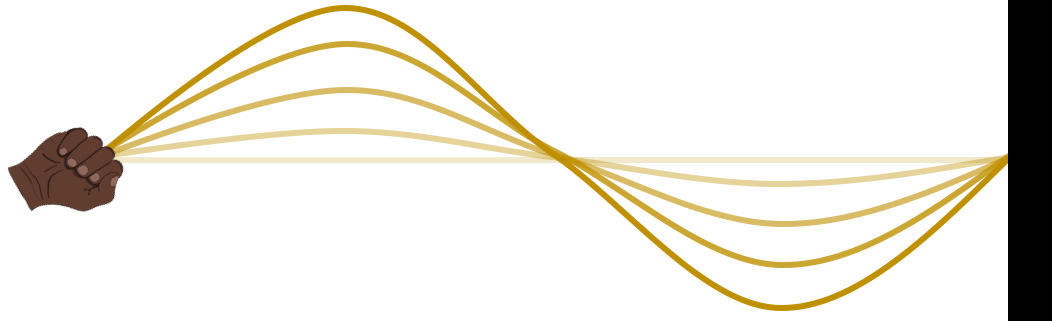
\includegraphics[width=0.7\linewidth]{files/standingwavetime-2308ee7c08556ff565c9b9dd4e91c9bf.png}
\caption[]{A standing wave as a stationary wave whose amplitude changes over time}
\label{fig:waves:standingwavetime}
\end{figure}

We can see from the equation that the maximum amplitude will be $2A$. This makes sense when we remember that the standing wave is made of two travelling waves of amplitude $A$. As these waves move, there will be moments when they completely constructively interfere, which is when the amplitude of the standing wave is maximized. When they completely destructively interfere, the amplitude is zero.
\end{framed}

\subsubsection{Summary}

A travelling wave is the propagation of a disturbance with a speed, $v$, through a medium. Particles in the medium oscillate back and forth, about an equilibrium position, as a wave passes through the medium, but they are not carried with the wave. Only energy is transmitted by a wave.

In a transverse wave, the particles in the medium oscillate in a direction that is perpendicular to the velocity of the wave. In a longitudinal wave, the particles of the medium oscillate in a direction that is co-linear with the velocity of the wave.

A sine wave is described by it frequency, $f$, its wavelength, $\lambda$, its amplitude, $A$, and its speed, $v$. We can also use the period of the wave, $T$, in lieu of the frequency. The frequency and wavelength of a wave are related to each other by the speed of the wave:
\begin{equation}
v = \lambda f
\end{equation}

Mathematically, a one-dimensional travelling sine wave moving in the positive $x$ direction can be described by:
\begin{equation}
D(x,t) = A \sin(kx-\omega t + \phi)
\end{equation}
where $D(x,t)$ is the displacement of the particle in the medium at position $x$ at time $t$. $\phi$ is the phase of the wave and depends on our choice of when $t=0$. $k$ is the wave number of the wave, and $\omega$ its angular frequency. These are related to the wavelength and frequency, respectively:
\begin{equation}
k &= \frac{2\pi}{\lambda}\\
\omega &= 2\pi f = \frac{2\pi}{T}
\end{equation}
If a dynamical model (e.g. Newton's Second Law) of a system/medium leads to an equation with the following form:
\begin{equation}
\frac{\partial ^2D}{\partial x^2}=\frac{1}{v^2}\frac{\partial ^2D}{\partial t^2}
\end{equation}
then waves with a speed of $v$ can propagate through the system/medium.

The speed of a wave on a rope of linear mass density, $\mu$, under a tension, $F_T$, is given by:
\begin{equation}
v=\sqrt{\frac{F_T}{\mu}}
\end{equation}

Generally, the speed of a wave in a medium depends on the elasticity of the medium when it is deformed and the inertia of the particles in the medium. In order for a wave to propagate through a medium, the particles in the medium must be able to be displaced from their equilibrium position.

A pulse travelling through a rope will get reflected at the end of the rope and travel back in the opposite direction. If the end of the rope is fixed, the reflected pulse will be inverted. If the end of the rope can move, the reflected pulse will be in the same orientation as the incoming pulse.

A one-dimensional wave in a rope of linear mass density, $\mu$, will transfer energy at an average rate:
\begin{equation}
P = \frac{1}{2}\omega^2\mu A^2 v
\end{equation}
A three dimensional spherical wave through a medium with density $\rho$ will transfer energy at an average rate:
\begin{equation}
P = 2\pi\rho\omega^2r^2 v
\end{equation}
at a distance $r$ from the source of the wave. The amplitude of a spherical wave will decrease as the distance away from the source increases:
\begin{equation}
A =\frac{1}{r}\sqrt{\frac{P}{2\pi\rho \omega^2 v}}
\end{equation}
The intensity of a spherical wave is defined as the power per unit area transferred by the wave, and is given by:
\begin{equation}
I=\frac{P}{4\pi r^2}=\frac{1}{2}\rho\omega^2A^2v
\end{equation}
The superposition principle states that if $D_1(x,t)$, $D_2(x,t)$, $\dots$, are functions that satisfy the wave equation, then any linear combination of these functions, $D(x,t)$:
\begin{equation}
D(x,t) = a_1D_1(x,t)+a_2D_2(x,t)+a_3D_3(x,t)+\dots
\end{equation}
will also satisfy the wave equation.

Different waves can interfere constructively or destructively in a medium, and the resulting wave is given by the sum of the functions describing the interfering waves.

Standing waves are formed when waves of the same frequency and amplitude travelling in opposite directions interfere. For standing waves on a string, the displacement of a particle on the string is given by:
\begin{equation}
D(x,t)=2A\sin\left(\frac{n\pi}{L}x\right)\cos(\omega t)
\end{equation}
where $n$ is the number of the harmonic and $L$ is the length of the string. In particular, a particle at position $x$ will move up and down as a simple harmonic oscillator with amplitude:
\begin{equation}
A(x) = 2A\sin\left(\frac{n\pi}{L}x\right)
\end{equation}
The condition for a standing wave to exist on a string is that the length of the string must be equal to a multiple of half of the wavelength of the standing wave:
\begin{equation}
L &= n\frac{\lambda}{2}\quad\quad n=1,2,3,\dots\\
\lambda &= \frac{2L}{n}\\
f &= \frac{nv}{2L}
\end{equation}

\begin{framed}
\textbf{Important Equations}\\
\textbf{Travelling 1d waves:}
\begin{equation}
D(x,t) &= A \sin(kx-\omega t + \phi)\\
k &= \frac{2\pi}{\lambda}\\
\omega &= 2\pi f = \frac{2\pi}{T}\\
v &= \lambda f
\end{equation}

\textbf{Wave equation:}
\begin{equation}
\frac{\partial^2D}{\partial x^2}=\frac{1}{v^2}\frac{\partial^2D}{\partial t^2}
\end{equation}

\textbf{Wave velocity:}
\begin{equation}
v=\sqrt{\frac{F_T}{\mu}} \quad v=\sqrt{\frac{E}{\rho}} \quad v=\sqrt{\frac{B}{\rho}}
\end{equation}

\textbf{Power (1d wave in a rope):}
\begin{equation}
P = \frac{1}{2}\omega^2\mu A^2 v
\end{equation}

\textbf{Spherical waves:}
\begin{equation}
P &= 2\pi\rho\omega^2r^2 v\\
A &=\frac{1}{r}\sqrt{\frac{P}{2\pi\rho \omega^2 v}}\\
I&=\frac{P}{4\pi r^2}=\frac{1}{2}\rho\omega^2A^2v
\end{equation}

\textbf{Standing waves:}
\begin{equation}
D(x,t)&=2A\sin\left(\frac{n\pi}{L}x\right)\cos(\omega t)\\
A(x) &= 2A\sin\left(\frac{n\pi}{L}x\right)
\end{equation}

\textbf{Standing waves on a string (both ends fixed):}
\begin{equation}
L &= n\frac{\lambda}{2}\quad\quad n=1,2,3,\dots\\
\lambda &= \frac{2L}{n}\\
f &= \frac{nv}{2L}
\end{equation}
\end{framed}

\begin{framed}
\textbf{Important Definitions}\\
\begin{itemize}
\item \textbf{Wavelength:} The distance between two successive maxima (``peaks'') or minima (troughs) in a wave. SI units: ${\rm \left[{m}\right]}$. Common variable(s): $\lambda$.
\item \textbf{Amplitude:} The maximal distance that a particle in a medium is displaced from its equilibrium position when a wave passes by. SI units: ${\rm \left[{m}\right]}$. Common variable(s): $A$.
\item \textbf{Frequency:} The number of complete oscillations in one second of a particle in a medium as a wave passes by. SI units: ${\rm \left[{s^{ -1}}\right]}$. Common variable(s): $f$.
\item \textbf{Bulk modulus:} A measurement of an object or substance's resistance to compression. SI units: ${\rm \left[{Pa}\right]}$. Common variable(s): $B$.
\item \textbf{Volume mass density:} The mass per unit volume of an object. SI units: ${\rm \left[{kg\cdot m^{ -3}}\right]}$. Common variable(s): $\rho$.
\item \textbf{Intensity:} The power per unit area transmitted by a wave. SI units: ${\rm \left[{W\cdot m^{ -2}}\right]}$. Common variable(s): $I$.
\end{itemize}
\end{framed}

\subsubsection{Thinking about the material}

\begin{framed}
\textbf{Reflect and research}\\
\begin{itemize}
\item Look up a video of the Tacoma Narrows bridge failing, and explain what happened.
\item Why do airlines ask you to turn off your electronic devices during take-off?
\item Is it true that there is no sound in space?
\item What type of wave was first observed in 2015?
\end{itemize}
\end{framed}

\begin{framed}
\textbf{To try at home}\\
\begin{itemize}
\item Confirm that the reflected pulse from a rope on a string is inverted when the end of the rope is fixed.
\item Think of different ways you could create a standing wave at home and try one of them out. How many harmonics can you create? How can you modify your set-up to create more harmonics?
\end{itemize}
\end{framed}

\begin{framed}
\textbf{To try in the lab}\\
\begin{itemize}
\item Propose an experiment to verify the relation $v=\lambda f$.
\item Propose an experiment which uses diffraction to measure small distances.
\item Propose an experiment to determine the chemical composition of the sun using a CD.
\item Design a device which acts as a echolocator and test its effectiveness in different scenarios.
\item Propose an experiment to observe triboluminescent x-rays produced by ripping scotch tape off of a surface.
\item Investigate and model refraction.
\item Investigate and model the doppler effect.
\item Investigate and model how standing waves behave on a stretched string, tube, or 2D medium.
\item Investigate and model audible beats.
\item Investigate and model double-slit interference.
\end{itemize}
\end{framed}

\subsubsection{Sample problems and solutions}

\paragraph{Problems}\label{sec:problemswaves}

\begin{framed}
\textbf{Problem 13.1}\\
A clarinet can be modelled as an air column that is open at one end and closed at the other end, as in Figure~\ref{fig:waves:clarinetmodel}.

\begin{figure}[!htbp]
\centering
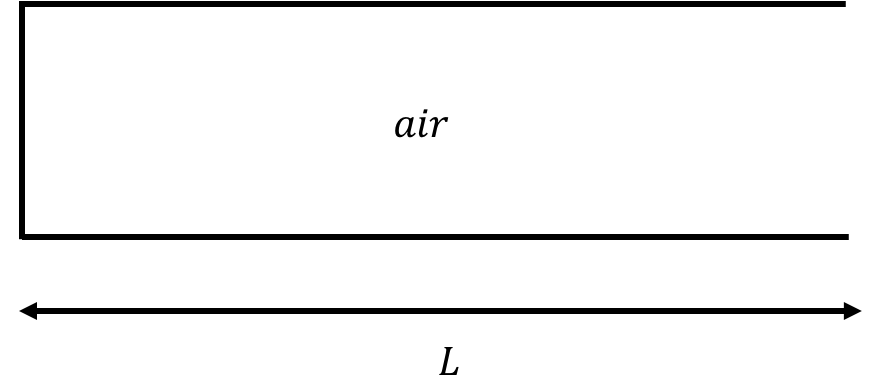
\includegraphics[width=0.5\linewidth]{files/clarinetmodel-8ed7d15265ce5f2a8af238d93b902b4e.png}
\caption[]{A clarinet (of length $L$) modelled as an air column that is closed at one end.}
\label{fig:waves:clarinetmodel}
\end{figure}

\begin{itemize}
\item a. Draw the first three harmonics for a clarinet (draw the maximum displacement of the air molecules as a function of distance in the clarinet).
\item b. Find an expression for the wavelength of the $n^{th}$ harmonic for a clarinet of length $L$.
\item c. If a clarinet is $60 {\rm cm}$ long, what is the lowest frequency note it can produce?
\end{itemize}
\end{framed}

\begin{framed}
\textbf{Problem 13.2}\\
A pulse propagates down a rope of mass per unit length $\mu_1$ that is tied to a second rope with a mass per unit length $\mu_2$ (Figure~\ref{fig:waves:reflectioncoeffgiven}). The tensions in the ropes are equal in magnitude.

\begin{figure}[!htbp]
\centering
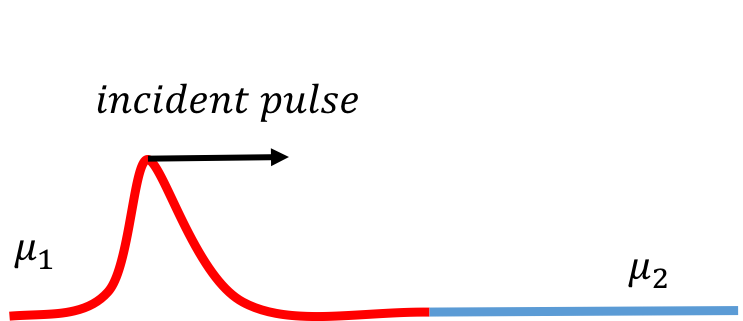
\includegraphics[width=0.5\linewidth]{files/reflectioncoeffgiven-307657fb762eb4d22dfac7c2f7aa29f3.png}
\caption[]{An incident pulse propagates through a rope connected to a another rope with a different linear mass density. When it reaches the boundary, part of the pulse will be reflected and part will be transmitted.}
\label{fig:waves:reflectioncoeffgiven}
\end{figure}

\begin{itemize}
\item a. Write the displacements of the incident pulse, the reflected pulse, and the transmitted pulse in the form $D(x,t)=D(a(t\pm x/v))$, where $a$ is some constant that you need to determine, and the choice of $+$ or $-$ depends on the direction that the pulse is travelling in.
\item b. The reflection coefficient, $R$, is the ratio of the amplitude of the reflected pulse to the amplitude of the incident pulse. Using the boundary conditions, show that the reflection coefficient is given by:
\end{itemize}
\begin{equation}
R=\frac{\sqrt{\mu_1}-\sqrt{\mu_2}}{\sqrt{\mu_1}+\sqrt{\mu_2}}
\end{equation}

Note: The boundary is the interface between the two ropes. By ``using the boundary conditions'', we mean that you should think about what must be true at the boundary for this problem to make sense. Boundary conditions are often more obvious than you think!
\end{framed}

\paragraph{Solutions}

\begin{framed}
\textbf{Solution 13.1}\\
\begin{itemize}
\item a. The first three harmonics are are shown in Figure~\ref{fig:waves:clarinet}.
\end{itemize}

\begin{figure}[!htbp]
\centering
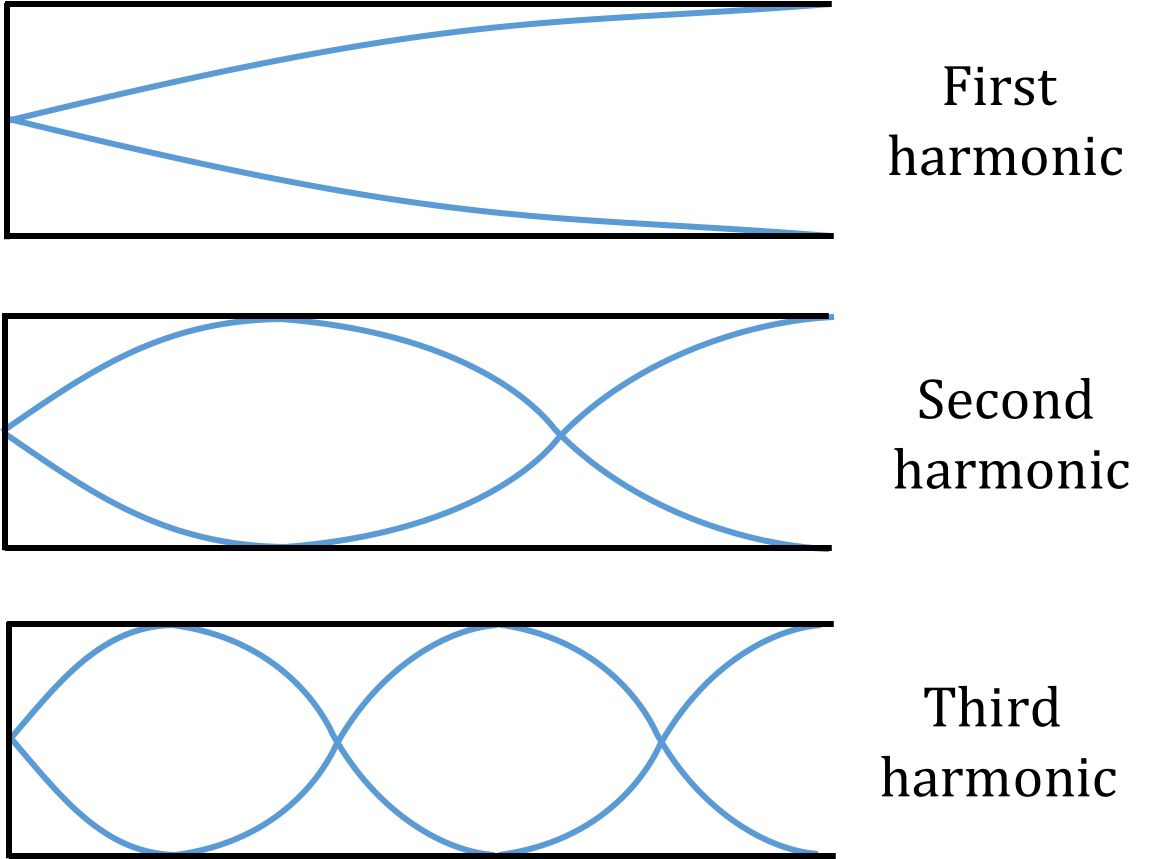
\includegraphics[width=0.5\linewidth]{files/clarinet-19b94846564ba9c3830f95308063cb65.png}
\caption[]{The first three harmonics for a clarinet. There is a node at the fixed end and an anti-node at the free end.}
\label{fig:waves:clarinet}
\end{figure}

\begin{itemize}
\item b. The equation for a standing wave is:
\end{itemize}
\begin{equation}
D(x,t)=2A\sin(kx)cos(\omega t)
\end{equation}
We let the fixed end be at $x=0$. At the fixed end, the displacement is equal to zero. At the free end ($x=L$) the displacement is maximized. The first condition is always true. The second condition will be met when:
\begin{equation}
\sin(kL)&=1\\
\therefore kL&=\pi/2,3\pi/2,...\\
\end{equation}
This condition can be expressed as:
\begin{equation}
kL&=\frac{(2n-1)\pi}{2}\\
\frac{2\pi L}{\lambda}&=\frac{(2n-1)\pi}{2}\\
\therefore \lambda&=\frac{4L}{2n-1}
\end{equation}
where, in the second line, we used $k=2\pi /\lambda$. We can check that this formula works for the first three harmonics:
\begin{equation}
n=1: \quad \lambda&=\frac{4L}{2(1)-1} \\
L&=\frac{1}{4}\lambda \\
n=2: \quad \lambda&=\frac{4L}{2(2)-1} \\
L&= \frac{3}{4}\lambda \\
n=3: \quad \lambda&=\frac{4L}{2(3)-1} \\
L&= \frac{5}{4}\lambda
\end{equation}
Referring back to our diagram (Figure~\ref{fig:waves:clarinet}), we can see that our formula holds true for the first three harmonics (i.e. for the first harmonic, the length of the clarinet is equal to $1/4$ of a wavelength, etc.)

\begin{itemize}
\item c. We found that the wavelength for the $n^{th}$ wavelength is given by:
\end{itemize}
\begin{equation}
\lambda=\frac{4L}{2n-1}
\end{equation}
Writing $\lambda$ in terms of the velocity, $v$, and frequency, $f$, gives:
\begin{equation}
\frac{v}{f}&=\frac{4L}{2n-1}\\
\therefore f&=\frac{v(2n-1)}{4L}
\end{equation}
From this formula, we can see that, if we want to find the lowest frequency, we want $n=1$. The length of the clarinet is $0.6 {\rm m}$, and $v$ is the speed of sound in air which is $343 {\rm m/s}$ at room temperature. Using these values, the lowest frequency is:
\begin{equation}
f&=\frac{(343 {\rm m/s})(2(1)-1)}{4(0.6 {\rm m})}\\
f&=143 {\rm Hz}
\end{equation}
Discussion: This frequency is close to the $D_3$ note, which has a frequency of $144 {\rm Hz}$, so this answer makes sense. However, the value we found differs from the true value. Why might this be?
\end{framed}

\begin{framed}
\textbf{Solution 13.2}\\
\begin{itemize}
\item a. We let the incident pulse move in the positive $x$ direction (Figure~\ref{fig:waves:reflectioncoeff}), and set $x=0$ to be where the ropes connect.
\end{itemize}

\begin{figure}[!htbp]
\centering
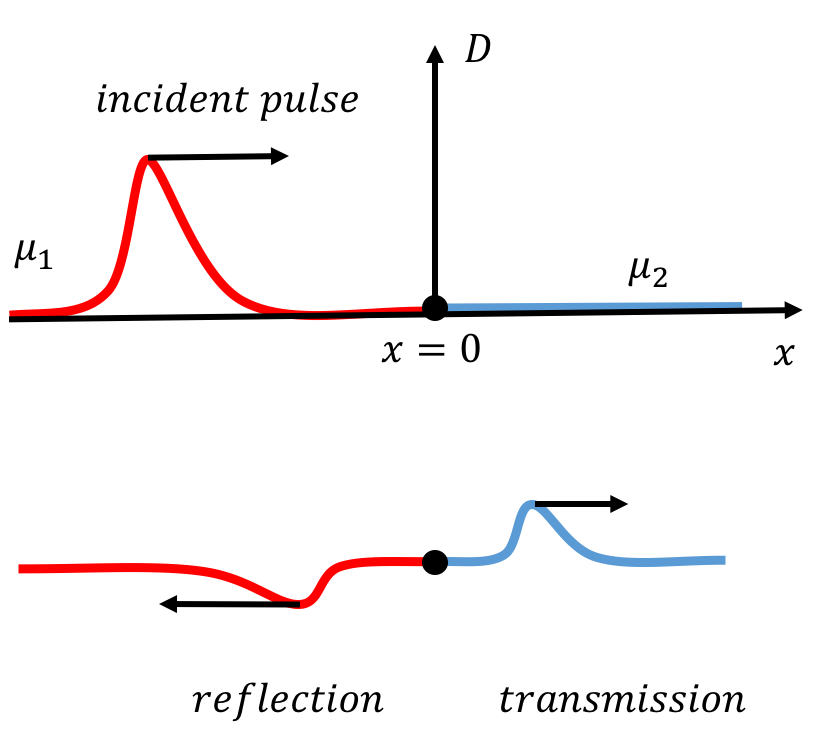
\includegraphics[width=0.5\linewidth]{files/reflectioncoeff-bfb79d9d186d5bb3a7da3d69c3a93760.png}
\caption[]{An incident pulse propagates through a rope connected to a another rope with a different linear mass density. When it reaches the boundary, part of the pulse is reflected and part is transmitted. Whether the reflected pulse is inverted or upright will depend on the reflection coefficient.}
\label{fig:waves:reflectioncoeff}
\end{figure}

The incident pulse (denoted by $i$) is a travelling wave, moving in one dimension in the positive $x$ direction. The incident pulse can thus be described by the function:
\begin{equation}
D_I(x,t)=A_I\cos(k_1x-\omega t)\\
\end{equation}
We will use the formulas $k=2\pi/\lambda$ and $\omega=2\pi f$ to rewrite this equation in the form $D=(a(t\pm x/v))$. The frequency, $f$, of the wave will be the same in both ropes. The velocity of the wave, and therefore its wavelength, depends on the mass density of the rope. Since the incident wave travels through the first rope ($\mu_1$), its velocity will be $v_1$ and its wavelength will be $\lambda_1$. The incident wave can thus be described by:
\begin{equation}
D_I&=A_I\cos\left( \frac{2\pi}{\lambda_1}x-2\pi ft\right)\\
&=A_I\cos \left( 2\pi\left(\frac{1}{\lambda_1}x- ft\right)\right)\\
&=A_I\cos \left( 2\pi f\left(\frac{x}{v_1}- t\right)\right)\\
&=A_I\cos \left( -2\pi f\left(t-\frac{x}{v_1}\right)\right)\\
D_I&=A_I\cos \left(2\pi f\left(t-\frac{x}{v_1}\right)\right)
\end{equation}
where we used $v=f\lambda$, and noted that $\cos( -x)=\cos(x)$.{\textbackslash}

The transmitted wave (denoted by the subscript $T$) will also travel in the positive $x$ direction, but its speed will be $v_2$, since it travels through the second rope:
\begin{equation}
D_T&=A_T\cos \left( 2\pi f\left(t-\frac{x}{v_2}\right)\right)
\end{equation}
The reflected wave (denoted by $R$) will travel in the $-x$ direction and at the same speed as the incident pulse.
\begin{equation}
D_R&=A_R\cos \left( 2\pi f\left(t+\frac{x}{v_1}\right)\right)
\end{equation}
\begin{itemize}
\item b. We will consider the boundary conditions at the interface between the two ropes. One boundary condition is that the rope must be continuous. As a result, the vertical displacement on the $-x$ side of the boundary must be the same as the vertical displacement on the $+x$ side of the boundary at every instant:
\end{itemize}
\begin{equation}
D_{-x}&=D_{+x}\quad\text{at $x=0$}
\end{equation}
The amplitude on the $+x$ side is equal to the amplitude of the transmitted pulse. For the $-x$ side of the boundary, we have to take into account that the incident and reflected pulses will superimpose (when the front of the incident pulse reaches the boundary, it will be reflected and interfere with the end of the incident pulse). This boundary condition can thus be expressed as:
\begin{equation}
A_I+A_R&=A_T
\end{equation}
The slope of the rope must also be continuous at the boundary. Since the incident and reflected pulses superimpose, and the principle of superposition states that the net displacement is the sum of the displacement of these two waves, we can write:
\begin{equation}
\frac{\partial}{\partial x}(D_I+D_R)\Bigr|_{x=0}=\frac{\partial}{\partial x}D_T\Bigr|_{x=0}\\
\frac{\partial}{\partial x}D_I\Bigr|_{x=0}+\frac{\partial}{\partial x}D_R\Bigr|_{x=0}&=\frac{\partial}{\partial x}D_T\Bigr|_{x=0}
\end{equation}
Using our equations for the incident, transmitted, and reflected pulses found in part a), and taking the appropriate partial derivatives, this equation becomes:
\begin{equation}
(A_I/v_1) \sin \left(2\pi f\left( t-\frac{x}{v_1}\right)\right)\Bigr|_{x=0}+(-A_R/v_1) \sin \left( 2\pi f\left( t+\frac{x}{v_1}\right)\right)\Bigr|_{x=0}&=\\(A_T/v_2) \sin \left( 2\pi f\left( t-\frac{x}{v_2}\right)\right)\Bigr|_{x=0}
\end{equation}
Evaluating at $x=0$ gives:
\begin{equation}
(A_I/v_1) \sin (2\pi ft) +(-A_R/v_1) \sin (2\pi ft)&=(A_T/v_2) \sin (2\pi ft)\\
\frac{A_I}{v_1} -\frac{A_R}{v_1}&=\frac{A_T}{v_2}
\end{equation}
Using our first condition, $A_I+A_R=A_T$, we get:
\begin{equation}
\frac{A_I}{v_1} -\frac{A_R}{v_1}&=\frac{A_I}{v_2}+\frac{A_R}{v_2}\\
\end{equation}
Now, we can rearrange to find the reflection coefficient, $R=A_R/A_I$:
\begin{equation}
A_I\left( \frac{v_2-v_1}{v_1v_2}\right)&=A_R\left( \frac{v_2+v_1}{v_1v_2}\right)\\
R&=\frac{v_2-v_1}{v_2+v_1}
\end{equation}
Since the velocities in the first and second rope are $v_1=\sqrt{F_T/\mu_1}$ and $v_2=\sqrt{F_T/\mu_2}$, respectively, the reflection coefficient can be written as:
\begin{equation}
R&=\frac{\sqrt{\frac{F_T}{\mu_2}}-\sqrt{\frac{F_T}{\mu_1}}}{\sqrt{\frac{F_T}{\mu_2}}+\sqrt{\frac{F_T}{\mu_1}}}\\
&=\frac{\sqrt{F_T}}{\sqrt{F_T}}\cdot \frac{\frac{1}{\sqrt{\mu_2}}-\frac{1}{\sqrt{\mu_1}}}{\frac{1}{\sqrt{\mu_2}}+\frac{1}{\sqrt{\mu_1}}}\\
\therefore R&=\frac{\sqrt{\mu_1}-\sqrt{\mu_2}}{\sqrt{\mu_1}+\sqrt{\mu_2}}
\end{equation}
as desired.
\end{framed}